%%%%%%%%%%%%%%%%%%%%%%%%%%%%%%%%%%%%%%%%%%%%%%%%%%%%%%%%%%%%
%%% LIVECOMS ARTICLE TEMPLATE FOR BEST PRACTICES GUIDE
%%% ADAPTED FROM ELIFE ARTICLE TEMPLATE (8/10/2017)
%%%%%%%%%%%%%%%%%%%%%%%%%%%%%%%%%%%%%%%%%%%%%%%%%%%%%%%%%%%%
%%% PREAMBLE
\documentclass[9pt,bestpractices,pubversion]{livecoms}
% Use the 'onehalfspacing' option for 1.5 line spacing
% Use the 'doublespacing' option for 2.0 line spacing
% Use the 'lineno' option for adding line numbers.
% The 'bestpractices' option for indicates that this is a best practices guide.
% Omit the bestpractices option to remove the marking as a LiveCoMS paper.
% Please note that these options may affect formatting.

\usepackage{lipsum} % Required to insert dummy text
\usepackage[version=4]{mhchem}
\usepackage{siunitx}
\DeclareSIUnit\Molar{M}
\usepackage[italic]{mathastext}
\graphicspath{{figures/}}

% added by DJS 2018/01/04
\usepackage{enumitem}
\usepackage{tabularx}
\usepackage{amsmath}
\usepackage{amssymb}
%\usepackage{subfig}
%\usepackage{subfigure}
%\usepackage{subcaption}

% added by DJS 2018/09/03
\usepackage{longtable}
%\usepackage{supertabular}

% added by DJS 2018/11/22
\setlist[itemize]{leftmargin=*}

%%%%%%%%%%%%%%%%%%%%%%%%%%%%%%%%%%%%%%%%%%%%%%%%%%%%%%%%%%%%
%%% IMPORTANT USER CONFIGURATION
%%%%%%%%%%%%%%%%%%%%%%%%%%%%%%%%%%%%%%%%%%%%%%%%%%%%%%%%%%%%

\newcommand{\versionnumber}{1.0}  % you should update the minor version number in preprints and major version number of submissions.
\newcommand{\githubrepository}{\url{https://github.com/davesmith4398/best_practice_membranes}}  %this should be the main github repository for this article

%%%%%%%%%%%%%%%%%%%%%%%%%%%%%%%%%%%%%%%%%%%%%%%%%%%%%%%%%%%%
%%% ARTICLE SETUP
%%%%%%%%%%%%%%%%%%%%%%%%%%%%%%%%%%%%%%%%%%%%%%%%%%%%%%%%%%%%
\title{Simulation Best Practices for Lipid Membranes [Article v\versionnumber]}

\author[1*]{David J. Smith}
\author[2*]{Jeffery B. Klauda}
\author[3*]{Alexander J. Sodt}
%\author[1,2\authfn{1}\authfn{3}]{Firstname Middlename Familyname}
%\author[2\authfn{1}\authfn{4}]{Firstname Initials Surname}
%\author[2*]{Firstname Surname}
\affil[1]{Department of Chemical Engineering, University of California, Santa Barbara, Santa Barbara, CA, USA}
\affil[2]{Department of Chemical and Biomolecular Engineering and Biophysics Program, University of Maryland, College Park, MD, USA}
\affil[3]{\textit{Eunice Kennedy Shriver} National Institute of Child Health and Human Development, National Institutes of Health, Bethesda, MD, USA}

\corr{djs01@umail.ucsb.edu}{DJS}  % Correspondence emails.  FMS and FS are the appropriate authors initials.
\corr{jbklauda@umd.edu}{JBK}
\corr{alexander.sodt@nih.gov}{AJS}

%\contrib[\authfn{1}]{These authors contributed equally to this work}
%\contrib[\authfn{2}]{These authors also contributed equally to this work}

%\presentadd[\authfn{3}]{Department, Institute, Country}
%\presentadd[\authfn{4}]{Department, Institute, Country}

\blurb{This LiveCoMS document is maintained online on GitHub at \githubrepository; to provide feedback, suggestions, or help improve it, please visit the GitHub repository and participate via the issue tracker.}

%%%%%%%%%%%%%%%%%%%%%%%%%%%%%%%%%%%%%%%%%%%%%%%%%%%%%%%%%%%%
%%% PUBLICATION INFORMATION
%%% Fill out these parameters when available
%%% These are used when the "pubversion" option is invoked
%%%%%%%%%%%%%%%%%%%%%%%%%%%%%%%%%%%%%%%%%%%%%%%%%%%%%%%%%%%%
\pubDOI{10.33011/livecoms.1.1.5966}
\pubvolume{1}
\pubissue{1}
\pubyear{2019}
\articlenum{5966}
\datereceived{13 June 2018}
\dateaccepted{27 November 2018}

%%%%%%%%%%%%%%%%%%%%%%%%%%%%%%%%%%%%%%%%%%%%%%%%%%%%%%%%%%%%
%%% ARTICLE START
%%%%%%%%%%%%%%%%%%%%%%%%%%%%%%%%%%%%%%%%%%%%%%%%%%%%%%%%%%%%

\begin{document}

\begin{frontmatter}
\maketitle

\begin{abstract}
%This particular document provides a skeleton illustrating key sections for a Best Practices document. Please see the sample \texttt{sample-document.tex} in \url{github.com/livecomsjournal/article_templates/templates} for additional information on and examples of using the LiveCoMS LaTeX class.
%Here we also assume familiarity with LaTeX and knowledge of how to include figures, tables, etc.; if you want examples, see the sample just referenced.

%In your work, in this particular slot, please provide an abstract of no more than 250 words.
%Your abstract should explain the main contributions of your article, and should not contain any material that is not included in the main text.
%Please note that your abstract, plus the authorship material following it, must not extend beyond the title page or modifications to the LaTeX class will likely be needed.
% JBK: I think we should not limit this to pure lipids...with CHARMM-GUI multicomponent is going to be the norm
We establish a reliable and robust standardization of settings for practical molecular dynamics (MD) simulations of pure and mixed (single- and multi-component) lipid bilayer membranes.
In lipid membranes research, particle-based molecular simulations are a powerful tool alongside continuum theory, lipidomics, and model, \textit{in vitro}, and \textit{in vivo} experiments.
Molecular simulations can provide precise and reproducible spatiotemporal (atomic- and femtosecond-level) information about membrane structure, mechanics, thermodynamics, kinetics, and dynamics.
Yet the simulation of lipid membranes can be a daunting task, given the uniqueness of lipid membranes relative to conventional liquid-liquid and solid-liquid interfaces, the immense and complex thermodynamic and statistical mechanical theory, the diversity of multiscale lipid models, limitations of modern computing power, the difficulty and ambiguity of simulation controls, finite size effects, competitive continuum simulation alternatives, and the desired application, including vesicle experiments and biological membranes.
These issues can complicate an essential understanding of the field of lipid membranes, and create major bottlenecks to simulation advancement.
In this article, we clarify these issues and present a consistent, thorough, and user-friendly framework for the design of state-of-the-art lipid membrane MD simulations.
We hope to allow early-career researchers to quickly overcome common obstacles in the field of lipid membranes and reach maximal impact in their simulations.

\begin{center}
	\begin{minipage}{.3\textwidth}
		\centering
		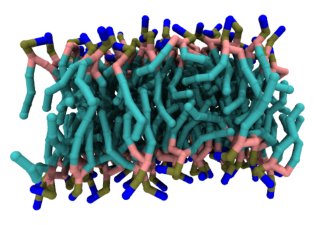
\includegraphics[width=\textwidth]{figures/bilayer_small.pdf}
	\end{minipage}%
	\begin{minipage}{.3\textwidth}
		\centering
		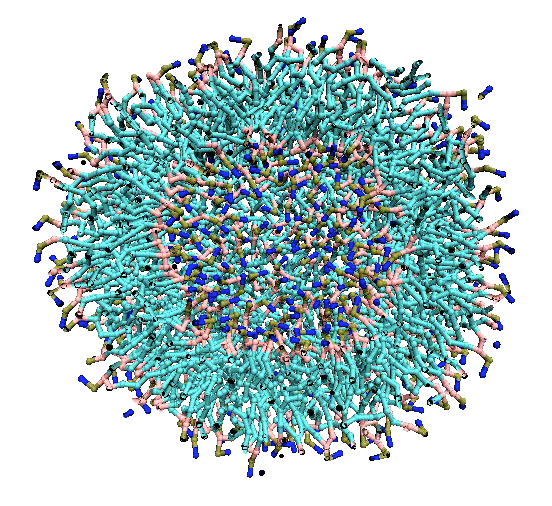
\includegraphics[width=\textwidth]{figures/vesicle_half_small.png}
	\end{minipage}%
	\begin{minipage}{.3\textwidth}
		\centering
		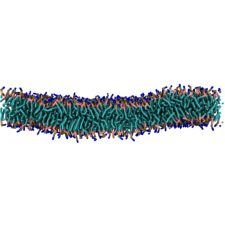
\includegraphics[width=\textwidth]{figures/bilayer_med.pdf}
	\end{minipage}
\end{center}

\end{abstract}

\end{frontmatter}

%%%%%%%%%%%%%%%%%%%%%%%%%%%%%%%%%%%%%%%%%%%%%%%%%%%%%%%%%%%%

\section{Introduction}
\label{sec:intro}
%Here you would explain what problem you are tackling and briefly motivate your work.
%In this particular template, we have removed most of the usage examples which occur in \texttt{sample-document.tex} to provide a minimal template you can modify; however, we retain a couple of examples illustrating more unusual features of our templates/article class, such as the checklists, and information on algorithms and pseudocode.

Lipid bilayer membranes have diverse applications in soft matter physics, pharmacology, and consumer products, and are first approximants to biological membranes.
Lipid bilayers are structures consisting of two molecularly-thick layers, or leaflets, on the scale of nanometers in aqueous solvent.
In these structures, molecules are oriented with their polar head groups pointing outward towards the solvent and their nonpolar tail groups pointing inward towards the other leaflet.
The dominant driving forces in their formation and stability include $(1)$ hydrophobic and dispersion interactions, wherein the lipid tail groups maximize their contacts with each other and minimize their contacts with water, decreasing area per lipid and $(2)$ head group electrostatic/excluded-volume repulsion and tail group conformational entropy, which work to increase the area per lipid ~\cite{Ben-Shaul1995}.

Generally, cylinder-shaped lipids form quasi-two-dimensional lamellae (macroscopic in two dimensions and nanoscopic in the third), while conical (larger headgroup) and inverse conical (smaller headgroup) lipid amphiphiles more favorably form micelles and inverted micelles, respectively ~\cite{Israelachvili2011}; however, this simple view of lipids has recently been of debate ~\cite{Sodt2016}.
Lamellar lipid bilayers often exist as multilayered vesicles, also known as liposomes--basically bilayer spheres--in solution, but can also exist in model experiments as planar bilayers across an aperture (black lipid membranes, or BLMs), laying on a solid support (supported lipid bilayers/SLBs), or directly anchored by a solid substrate (tethered bilayer lipid membranes/t-BLMs).
For experimental analysis of lipid membranes, bilayers are normally assembled in multilayered stacks, while in simulations, lipid membranes are often studied as planar bilayers with periodic boundary conditions.

There is an extensive continuum theoretical framework for lipid bilayer membranes.
Lamellar lipid membranes are interfaces embedded in three dimensions, but are more complicated than typical liquid-liquid interfaces due to their finite thickness and preferred area per molecule depending on the lipids' molecular neighbors and composition ~\cite{Diamant2011,Safran1994}.
They also differ from solid-solid interfaces, due to their negligible surface tension.
Because of these complexities, simple interfacial theories of surface tension in terms of, e.g., an oil-water interface or even an interface with capillary fluctuations are often insufficient for membranes.
Alternatively, fluid (liquid crystalline) lipid membranes are normally modeled as liquid-like laterally (without an in-plane shear modulus), and solid-like transversely (out-of-plane).

Another major continuum assumption is that the lipids are strongly surface active, and therefore are not soluble in bulk aqueous solvent ~\cite{Safran1994}.
In aqueous solution, the lipids thus form a macroscopic interface where the head groups maintain contact with the water and the tail groups are buried, in contact with each other.
In a rectangular thermal system of constant size, i.e. the canonical ensemble, the system may reach a point where the lipid-water interface is ``saturated,'' i.e. the lipids are packed on average at their optimal area per molecule.
Since the addition of more lipids would further decrease the average area per molecule to an extent that may be globally unfavorable or higher total free energy, the membrane may instead ``buckle,'' curving the lipid-water interface to accommodate additional lipids at the same average area per molecule.
In a system of constant tension, the addition of more lipids will instead expand the area of a bilayer that on average is flat.

For continuum lipid bilayer physics, it is almost always safe to assume volume incompressibility, as negligible fluctuations in volume cost far more than typical thermal fluctuations ~\cite{Safran1994,Sundararajan2008}.
Area incompressibility is a less common assumption and invalid in many cases; however, area fluctuations are often assumed to exchange with thickness or peristaltic fluctuations through a simple equation of state whereby area and thickness are inversely correlated ~\cite{Safran1994}.
For this reason, a Gibbs monolayer or two-dimensional surface description is a common and often reasonable theoretical approach.
Perhaps the most studied fluctuations in lipid membranes, and what separates them from most conventional solid-liquid and liquid-liquid interfaces, are in mesoscopic shape, termed undulations ~\cite{Canham1970b,Helfrich1973a}.
This is typically approached from the perspective of membrane curvature elasticity, where large wavelength bending modes are highly accessible via thermal fluctuations.
These out-of-plane modes lead to a distinction between the projected (in-plane, or $xy$) area and contour area (that of the 3D membrane surface); therefore, care should be taken in deconvoluting deformations in membrane curvature or bending from those in contour area or expansion/compression.
Still, other fluctuations are accessible at smaller length scales, and typically involve local lipid orientation or ``tilt'' relative to mesoscopic shape and operations thereof, as in other liquid crystalline systems ~\cite{Hamm2000,May2007,Watson2011a,Watson2013b}.

Despite the extensive physical framework for lipid bilayer membranes from both continuum theory and experiments, detailed molecular simulations can be a tremendous asset to a further understanding.
Molecular simulations were first applied to lipid membrane systems in the early 1990s, and have since become increasingly amenable to larger spatiotemporal scales and higher resolutions ~\cite{Venable2015}.
In general, molecular simulations work well for lipid membrane studies in the following instances:
\begin{itemize}
	\item When nanometer resolution is required, and chemical detail is important, e.g. for heterogeneous membranes, and in the case of additional non-lipid components
	\item For finite-sized systems where macroscopic continuum principles may not apply
	\item For a detailed view of thermal fluctuations and the role of entropy
	\item When the interior of the membrane is being probed, and the two-dimensional/thin film assumption is not a given
	\item To verify a mesostructure (lamellae, hexagonal phases, etc.) that is well characterized by experiments and continuum theories, or determine the mesostructure when it is in fact unclear
	\item To test continuum mechanical assumptions, e.g. volume/area compressibility, tension, bending renormalization, structure of pores, etc.
	\item To parameterize continuum theory and simulations, i.e. with spatiotemporal and macroscopic properties)
\end{itemize}

If any of the above conditions are met, the researcher should consider the utility of molecular simulations.
Before diving into molecular simulations of lipid membranes, we emphasize the utmost importance in formulating a specific scientific question that can be addressed with the simulations, then designing the simulation framework accordingly.
Example scientific questions include:

\begin{itemize}
	\item What is the activation barrier and rate of membrane pore formation and closure?
	\item How does lipid leaflet number asymmetry relate to membrane curvature?
	\item What is a reasonable bending modulus to plug into a continuum theoretical simulation of a complex, multicomponent membrane?
	\item How does phase separation facilitate morphological transformations in lipid vesicles?
\end{itemize}

Simulations can also supplement experiments, for driving questions such as:

\begin{itemize}
	\item What is the phase behavior of a ternary mixture of lipids at a particular temperature  and composition?
	\item What is the membrane flux of water, of a particular ion/drug, a nanoparticle, peptide, or any molecule?
	\item How does a particular membrane protein fold and mediate membrane structure?
	\item Does cholesterol make a particular membrane more or less fluid?
	\item For a particular membrane, what is the rate of lipid flip-flop?
	\item How does natural lipid diversity influence bilayer structure and function?
\end{itemize}

In the recommendations that follow, we lay out guidelines for robust and reproducible equilibrium simulations of lipid bilayer membranes.
We focus on dilute lamellar bilayer membranes in water, i.e. at high hydration, particularly the membrane fluid (liquid-crystalline, $L_\alpha$) phase and, where relevant, gel ($L_\beta$ or $L_{\beta '}$) and liquid-ordered ($L_o$) phases.
While we do not dictate the choice of MD package for simulation, we draw heavily on tools available in the GROMACS package ~\cite{VanDerSpoel2005}, which has several built-in routines and add-on patches  ~\cite{Buchoux2017,Lukat2013,Truhlar2009a} and is the default for several multiscale lipid membrane models ~\cite{Poger2010a,Jambeck2012,Marrink2004,Marrink2007a,Arnarez2015}.
NAMD ~\cite{Phillips2005}, CHARMM ~\cite{Gumbart2007}, and AMBER ~\cite{Case2018} are well established for lipid membrane simulations as well.
Where direct reading, writing, and analysis of the MD trajectories is deemed necessary, we recommend the Python-based packages \textit{MDTraj} (\url{http://mdtraj.org/}) and \textit{MDAnalysis} (\url{https://www.mdanalysis.org/}).

%%%%%%%%%%%%%%%%%%%%%%%%%%%%%%%%%%%%%%%%%%%%%%%%%%%%%%%%%%%%

\section{Prerequisites}
\label{sec:prereq}
%Here you would identify prerequisites/background knowledge that are assumed by your work and your checklist which you view as critical, ideally giving links to good sources on these topics.
%Checklists are normally focused on errors made by users with training and experience in molecular simulations, so you can assume a basic familiarity with the fundamentals of molecular simulations.
Some good textbooks for statistical mechanical and thermodynamic background on membranes include:

\begin{itemize}
	\item Safran, Samuel A. ``Statistical Thermodynamics of Surfaces, Interfaces, and Membranes.'' 2003: Westview Press.
	\item Nelson, David R., et al. ``Statistical Mechanics of Membranes and Surfaces.'' 2004: World Scientific Publishing Company.
	\item Boal, David. ``Mechanics of the Cell.'' 2012: Cambridge University Press, New York.
\end{itemize}

Good papers and textbooks for computational and simulation guidance on membranes include:

\begin{itemize}
	\item Sundararajan, V. ``Computational Modeling of Membrane Bilayers, Volume 60 (Current Topics in Membranes).'' 2008: Academic Press.
	\item Tieleman, Marrink, and Berendsen. \textit{Biochimica et Biophysica Acta,} 1997.
\end{itemize}

In this article, we also assume basic proficiency with MD simulation. Where necessary, we refer simulators to other best practices documents for introductory guides:

\begin{center}
	\begin{minipage}{\columnwidth}
		\centering
		\begin{itemize}
		\item MD basics \url{https://github.com/MobleyLab/basic_simulation_training}
		\item MD setup, biomolecular setup \url{https://github.com/michellab/BioMolSetupPaper}
		\item Transport properties \url{https://github.com/ejmaginn/TransportCheckList}
		\item Statistical error and uncertainty analysis \url{https://github.com/dmzuckerman/Sampling-Uncertainty}
		\end{itemize}
	\end{minipage}%
\end{center}

%%%%%%%%%%%%%%%%%%%%%%%%%%%%%%%%%%%%%%%%%%%%%%%%%%%%%%%%%%%%

\section{Checklist}
\label{sec:checklist}
%Your checklist should include a succinct list of steps that people should follow when carrying out the task in question.
%This is provided to ensure certain basic standards are followed and common but critical major errors are avoided.
%Note that a checklist is not intended to cover \emph{all} important steps, but rather focus on the most common reasons for failure or incorrect results, or issues which are particularly crucial.
%Here we use a full-page checklist with multiple sections, so it will appear on a separate page of the sample PDF.
%Other checklist formats are possible, as shown in the sample \texttt{sample-document.tex} in \url{github.com/livecomsjournal/article_templates/templates}.
In this section, we provide a checklist for the four major steps in the lipid membrane simulation process: (1) model selection, (2) pre-simulation considerations, including selection of MD settings, (3) preparation of initial configurations, and (4) post-simulation considerations, including validation of calculated properties.

\subsection{Model selection}
\label{subsec:models3}
As with other systems, model selection for lipid membranes is crucial.
Lipid membrane models are relatively diverse--resolution can range from all-atom to united atom to coarse-grained and from explicit to implicit solvent.
Furthermore, the lipid model may ultimately be implicated in some more complicated application, e.g. small solute transport, peptide-induced pore formation, embedded proteins.
The model selection process for a given physical problem can at times be daunting, especially for an undergraduate, experimentalist, or otherwise newcomer.

The main goal for a lipid membrane model study should be to correctly capture the relevant structural, mechanical, thermodynamic, and/or dynamic properties.
Furthermore, these properties should be accurate at the relevant length and timescales and the correct equilibrium conditions (thermodynamic, temperature, pressure, etc.) and/or nonequilibrium conditions (thermal/mechanical/chemical/other gradients).
However, accuracy must be balanced with efficiency.
Generally speaking, the simulation time $t_{sim}$ is a function of the (1) model, (2) system size, (3) computing resources, and (4) MD package, amongst other factors.
These contributions are often overlapping, but can be deconvoluted in some simple scaling laws; cf. Section~\ref{subsec:models4} for more details.

In general, force field developers seek to first capture structural and thermodynamic properties, then address dynamical properties.
This balance can be tricky, especially with all-atom force fields, as parameters that work for thermodynamics may not accurately match dynamical properties.
Rigorous models are validated via their properties through experimental comparison, and with the proper corrections and normalization, the most important of which are finite size effects in periodic simulations  ~\cite{Venable2017,Klauda2006b}.
The discussion of model selection, including a comprehensive survey of force fields with their advantages and disadvantages and at various resolutions, is continued in Section~\ref{subsec:models4} after the definition and discussion of membrane properties to facilitate the most informed decision making for the reader.

\subsection{Pre-simulation considerations, including selection of MD settings}
\label{subsec:presim3}
Once the model is selected, the pre-simulation considerations mainly concern the thermodynamic conditions under which the membrane simulation is ultimately going to be run.
Proper control over membrane phase behavior and mechanical tension often necessitates the use of thermostats and barostats.
The relevant thermodynamic ensembles for the study of lipid membranes are the canonical ($NVT$), isobaric/isothermal ($NPT$), and multiphase ($NP_z \gamma T$) ~\cite{Devireddy2010} ensembles.
Here, $P_z$ is the pressure in the transverse or membrane out-of-plane direction.
We describe the tension $\gamma$ in more detail below.
Assuming a well-tuned force field, we recommend the simulation of planar bilayers with equal planar dimensions ($x=y$) in the semi-isotropic $NP_{z}P_{xy}T$ ensemble, where $P_{xy} = P_x = P_y$ is pressure in the lateral or membrane in-plane directions.
Alternatively, the $NVT$ ensemble may be required to avoid cell dimension fluctuations, or the $NP_z \gamma T$ ensemble may be required to probe the effect of surface tension.

The target temperature should be guided by the experimental correspondence.
For the ideal model, the simulation temperature would be set to match that of experiment.
In reality, however, the imprecise energy-entropy breakdown in the membrane model may lead to shifted phase transition temperatures, and therefore the need to simulate at a higher or lower temperature, depending on the desired membrane phase.
Force fields like CHARMM36 ~\cite{Klauda2010d} are well-tuned for phase changes within $5^o$C, which has been determined through thorough simulations at a single temperature, i.e. without dynamical ramping of temperature ~\cite{Khakbaz2018}.
The main transition temperature of interest is the gel-to-liquid phase transition temperature $T_g$, above which the membrane exists in a disordered liquid crystalline $L_\alpha$ state and below which the membrane exists in a more ordered gel $L_\beta$ state.
Some models may accurately capture intermediate tilted gel $L_{\beta '}$, ripple $P_{\beta '}$, and interdigitated $L_{\beta I}$ phases whose relevance depends on the experiments you are trying to model.
Most simulations approximate a cellular membrane as a fluid lipid bilayer to match biological conditions, and build chemical and mechanical heterogeneity in later.

For the isobaric/isothermal and multiphase ensembles, pressure control will additionally be required.
For membranes in the isobaric/isothermal ensemble, pressure control is often conducted in a semi-isotropic scheme ($NP_{z}P_{xy}T$) to ensure consistent scaling in the bilayer plane, independent of the out-of-plane dimension.
For membranes, the definition of tension is a precarious one that might not be trivial to a newcomer.
The frame tension $\tau$, conjugate to the membrane projected area $A_p$, is the force per unit length exerted at the edges of the simulation box, and therefore the force per unit length required to maintain $A_p$ ~\cite{Diamant2011}.
The Laplace tension $\gamma$, conjugate to the membrane fluctuating contour area $A$, is the response of the membrane to out-of-plane strain ~\cite{Diamant2011}.
The Laplace tension is defined to a first approximation as ~\cite{Kirkwood1949}:

\begin{equation}\label{eq:1}
	%\label{e:partition}
	\gamma =0.5 L_z\big(P_z-P_{xy}\big)
\end{equation}
where $L_z$ is the transverse length scale, in the membrane out-of-plane direction.
While there is an important distinction between $\tau$ and $\gamma$, it has been clearly shown through thermodynamic arguments that these tensions and their corresponding areas are directly related, and therefore not independent ~\cite{Diamant2011}.
For a stress-free membrane, one whose area per molecule is allowed to relax to the imposed tension, $\tau = (A/A_p) \gamma$ ~\cite{Diamant2011}.
Thus, both tensions reduce to zero when the component pressures are set to be equal.
Furthermore, under positive tension (area expansion of the membrane), $A$ and $A_p$ are roughly equal and $\tau \approx \gamma$ in this case as well.
In this document, we therefore refer to $\gamma$ as the tension controlled in simulation, which is controlled by setting $P_{z}$ and $P_{xy}$.
Since experimental and biological membranes often operate at negligible tension--as their conjugate variable, the area per lipid, is unconstrained and therefore used to minimize the free energy--tensionless membranes are currently the most common.

In general, most other MD settings should be chosen appropriately for the chosen force field and simulation package.
For a discussion of appropriate simulation settings, see Section~\ref{subsec:presim4} and \url{https://github.com/MobleyLab/basic_simulation_training}

\subsection{Preparation of initial configurations}
\label{prepconf3}
Lamellar lipid bilayers exist for a variety of concentrations of water to lipid ratios.
All force fields will produce bilayers if conditions are at full hydration ($\sim$30 waters per lipid) or above.
For a planar bilayer, the desired number of lipids or membrane size in the $xy$-plane can be estimated from one another if the area per lipid is roughly known:

\begin{equation}\label{eq:2}
	%\label{e:partition}
	N_l = \frac{2 L_x L_y}{a_l}\ \quad (planar)
\end{equation}
where $N_l$ is the total number of lipids, $L_x$ and $L_y$ are the lateral box dimensions in the $x$ and $y$ directions, and $a_l$ is the area per lipid.
The factor of two comes from the fact that there are two leaflets.
If a mixed lipid component bilayer, then the $a_l$ is the composition-weighted average.
The amount of solvent can be independently varied by changing the box $z$-dimension $L_z$. The number of solvent molecules can be estimated from the following:

\begin{equation}\label{eq:3}
	%\label{e:partition}
	N_{solv} = L_x L_y (L_z - D_B) \rho_{solv} \quad (planar)
\end{equation}
where $N_{solv}$ is the number of solvent molecules, $D_B$ is the bilayer thickness, and $\rho_{solv}$ is the estimated or known bulk number density of the solvent model.

Similarly, for a vesicle, the number of lipids/membrane size and amount of solvent can be estimated via:

\begin{subequations}\label{eq:4}
\begin{align}
N_l = \frac{8 \pi R^2}{a_l}\ \quad (vesicular)\label{eq:4a} \\
N_{solv} = (L_x L_y L_z - 4\pi R^2 D_B) \rho_{solv} \quad (vesicular)\label{eq:4b}
\end{align}
\end{subequations}
where $R$ is the vesicle radius defined from the center to the bilayer midplane.
It is important to note that the leaflet lipid numbers will be equal and the above equations will be exact only in the limit of an infinitely large vesicle.
For finite-sized vesicles and especially nanoscale ones, the inner leaflet lipid number will be significantly lower than that of the outer leaflet, and the above equations will break down.
In this scenario, membrane builder programs like \textit{CHARMM-GUI} can be of assistance.

For a vesicle, the total membrane area must be smaller than the smallest plane in periodic box; otherwise, the lipids will form a planar bilayer to minimize the free energy.
The cost of forming a vesicle from a planar membrane incurs at least a bending and Gaussian curvature energetic penalty.
Furthermore, simulating a membrane area smaller than the smallest plane in the periodic box does not ensure the formation of a stable vesicle; in fact, a pancake structure or bilayer patch with splayed edges can be more stable up to a critical size on the order of a 10 nm radius, and therefore $10^3$ to $10^4$ total lipids ~\cite{Deserno2009}!

\subsubsection{Membrane construction}
\label{subsubsec:construction}
Once the number of lipids and solvent molecules and periodic box dimensions are determined, there are two main methods for putting them all together: (1) ``templating'' and (2) self-assembly. These two methods are introduced below, and are further discussed, along with alternatives, in Section~\ref{subsec:prepconf4}.

In the templating method, the lipids are pre-arranged in a planar or vesicular bilayer, close to the final equilibrated structure.
We recommend the use of existing templating packages and routines, due to the potential of core overlaps for both planar and vesicular bilayers and for the desired leaflet number asymmetry for vesicles, especially at smaller radii.
\textit{CHARMM-GUI} (\url{http://www.charmm-gui.org/}) is an excellent resource, and the most common for setting up membranes in a variety of configurations and for a variety of models/force fields  ~\cite{Jo2009,Cheng2013,Wu2014,Brooks2009}.
\textit{CHARMM-GUI} provides input files compliant with the GROMACS, NAMD, AMBER, OpenMM, and CHARMM MD packages, amongst others, but is limited in force fields to CHARMM36 ~\cite{Javanainen2016} and the Martini force fields ~\cite{Qi2015a}.
Once the membrane is templated, it can then be solvated.
Due to the fluctuating nature and molecular scale roughness of lipid membranes, a trial-and-error solvation routine placing test particles in various locations, checking for steric overlap based on van der Waals radii, and removing particles if overlap is significant, may be preferred over appending solvent ``slabs'' to each side of the membrane due to the potentially long equilibration time of full head group solvation.
The GROMACS \textit{g\_solvate} routine is one such example of a trial-and-error approach, whereas \textit{CHARMM-GUI} uses a slab-based approach.

In the self-assembly method, the lipids are dispersed in solvent, and allowed to dynamically and spontaneously arrange into their final equilibrium structure.
The initial stages are normally fast, and involve the formation of lipid micellar aggregates followed by the bridging of micelles to form larger, lamellar aggregates.
The rate-limiting step is believed to be the elimination of water pores in the membrane, sealing over $10$ to $10^2$ ns during which lipids may exchange across leaflets ~\cite{DeVries2004}.
The proof-of-concept approach is more scientifically satisfying, but not necessarily reasonable for higher resolution models and/or larger length scale simulations due to the long time scale of assembly.
These matters are discussed more in Section~\ref{subsubsec:prepproc}.
Again, care should be taken to generate a vesicle or bilayer, and not a pancake or other structure.
Because the system will always proceed to minimize its total free energy, the initial box dimensions are crucial to the outcome of the self-assembly approach.
For a planar bilayer, the in-plane box dimensions must be initialized near their intended end state--which can be predicted with the number of lipids and area per lipid--and for a vesicle, all box areas must be significantly larger than the corresponding planar bilayer with the same number of lipids; otherwise, the lipids will form a planar bilayer and not a vesicle.
For one example of the self-assembly technique, you can visit the Martini website (\url{http://www.cgmartini.nl/index.php/tutorials-general-introduction-gmx5/bilayers-gmx5}).

\subsubsection{Preparation procedure}
\label{subsubsec:prepproc}
After the building step, the system should be energy minimized to remove potential bad site contacts or steric overlap generated during the original placement of molecules.
Minimization routines like steepest descent are perfectly reasonable, and are available in conventional MD packages.

Then, the system should be gradually annealed from 0~K to the target temperature in the relevant thermodynamic ensemble ($NVT$ or $NP_{z}P_{xy}T$, depending on whether or not a barostat will ultimately be used in the production run).
In general, a short 100 ps to 1 ns run should suffice.
The user may want to consider using position restraints during this process to prevent major lipid fluctuations, particularly if the templating method is used to initially build the bilayer.
For \textit{CHARMM-GUI}, we recommend using its equilibration scripts, which have been extensively tested on various bilayers.
For soft enough interactions, you may be able to skip this step.

In the case of self-assembly, a longer dynamical simulation is needed to allow for bilayer formation.
For smaller, $\approx$ 128-lipid membranes, this can take 10-100 ns, and can potentially take much longer for larger and vesicular ones.
Visualization can be very helpful to track the assembly process.
Care should still be taken after assembly is qualitatively confirmed to ensure quantitative equilibration.

Before the production run, the equilibrium structure can be further standardized for ease of analysis and comparison with external studies.
Out of convention, for an open planar membrane, the membrane in-plane directions are often defined to be the $x$ and $y$ directions, while the out-of-plane direction is defined as $z$.
All subsequent discussion assumes this directionality, but the choice of direction is otherwise arbitrary.
In GROMACS, this can easily be achieved with the $editconf$ command.
For both open planar and closed vesicular membranes, centering the membrane in the periodic box will largely prevent the jumping of bilayer leaflets and pieces across the periodic box, assuming drift does not occur.
This will make subsequent visual observation and post-simulation analysis easier.
Centering can also be achieved with $editconf$.

Before going into the details of production run, it should be noted that additional equilibration beyond the initial structure is needed and timescales depend strongly on the system complexity and size.
For single-component lipid membranes in the liquid crystalline state, equilibration typically only requires 5-10 ns with a well educated initial setup of surface area per lipid.
Membranes that have several lipids or conditions in more condensed phases can require 100+ ns of equilibration; the exact amount of time, however, will depend strongly on the composition and whether or not phase segregation is relevant.
A typical first order method to determine equilibration is to track surface area per lipid as a function of time and verify that this has reached equilibrium via block averages and autocorrelation analysis ~\cite{Venable2015}.
However, all other key properties should also be verified--i.e., that they have stabilized and that reported averages are over equilibrated systems.
This is especially true for lipid lateral clustering and radial distribution functions that depend on slowly relaxing diffusional degrees of freedom.

\subsubsection{Guidelines for production run sampling}
\label{subsubsec:prodrun}
Finally, the initial estimation of the production run time is useful.
You will ultimately want to incorporate an adequate amount of sampling for your phenomenon/phenomena of interest.
In general, this means capturing several autocorrelation times for the relevant degrees of freedom.
Lipid membranes are characterized by a hierarchy of time scales, including: bond vibrations (fs-ns), trans-gauche isomerization and rotation about chemical bonds (1-100 ps), rotation or axial diffusion about the lipid axis and wobbling (1-100ns), lateral diffusion (1-100 $\mu$s), and flip-flop (1 ms-1 s for most lipids ~\cite{Vermeer2007,Konig1996,Leftin2011}; shorter for cholesterol) and undulations (1 ms-1 s for experimental system sizes ~\cite{Vermeer2007} and down to $\sim$100 ns-1 us for typical simulation ~\cite{Bochicchio2016}).
Collective order fluctuations such as undulations, flip-flop, lateral diffusion are the longest timescale fluctuations in the system because they involve the coordination and motion of several lipids  ~\cite{Vermeer2007}.
Even at equilibrium, area per lipid can fluctuate in simulations on the time scale of tens of nanoseconds  ~\cite{Poger2016,Venable2015}.
However, if your study concerns more localized or molecular degrees of freedom such as rotation about chemical bonds, trans-gauche isomerization, and lipid axial diffusion at constant membrane macroscopic shape and lipid leaflet number, then smaller sampling times may be permissible.

\subsection{Post-simulation considerations, including validation of calculated properties}
\label{subsec:postsim3}
Fluid lipid membranes are normally modeled as liquid-like laterally, without an in-plane shear modulus, and solid-like transversely.
Because of this, important properties to verify include in-plane structure, elasticity, and dynamics and out-of-plane structure and elasticity.

It is the responsibility of computationalists in the field of membranes and otherwise to adequately validate the physical properties resulting from their model.
Wherever possible, properties calculated in simulation should be compared with experiment.
One particularly good reference for rough property estimates is from the work of Phillips ~\cite{Phillips2017}.
Experimental reference data can be classified as either direct or indirect.
Direct data includes experimentally measured properties like x-ray and neutron form factors from scattering experiments and the NMR bond order parameter, while indirect data includes properties inferred from direct experimental data based on a given theoretical model like the area per lipid, the bilayer thickness, and the lipid diffusion coefficient.
Ideally, force field and simulation validation should be based on the comparison of simulated data with direct experimental data, but this is not always possible ~\cite{Poger2016}.
Therefore, we discuss both types of data comparisons.
The method of calculation in experiment does matter to the method of calculation in simulation.
For example, methods based on biased membrane perturbations may deviate significantly from those based on equilibrium fluctuations such as micropipette aspiration versus flicker experiments ~\cite{Venable2015}.
Wherever possible, the theoretical basis for both the experimental and simulation property calculations should be used as a guide.

If the property computed in simulation is out-of-line with the expectation from experiment, it is crucial to consider the meaning of the discrepancy.
Assuming that your model was properly selected to reproduce the properties that you wish to capture, the first step we recommend is to verify the settings and preparation procedure of your simulation.
There may be some differences between your simulated system and that of experiment--for example, in composition of lipids, ions, or other inhomogeneities like proteins.
In this case, it may be scientifically fruitful to pursue the difference in systems further; otherwise, the simulated system should be tweaked to more closely match the conditions in experiment.
If the systems in simulation and experiment are expected to be identical, the simulator should strive for the best possible statistics in the simulation production run, for increased confidence that property values should indeed agree.
A final point is that experimental results are not infallible.
When simulation and experiment do not agree or there is large variation within experimental measurements for the same property and the computational procedure is sound, simulations can provide refinement to the experimental results ~\cite{Venable2015}.

Perhaps the most important verification of any lipid membrane model involves the continuous structural and mechanical profiles in the out-of-plane or ``transverse'' $z$ direction. The lipid bilayer membrane's internal structure and mechanics are crucial to its physics. These metrics include (1) the local density profile and (2) the stress profile.

\subsubsection{Transverse local density profile}
\label{subsubsec:locdens}
As for general liquid-liquid interfaces, the density profile $\rho(z)$ is a crucial structural metric for lipid bilayer membranes.
A typical transverse local electron density profile is shown in Figure~\ref{fig:density}.
Various regional models have been proposed to characterize the membrane based on its component and overall densities.
For atomistic models, the local density profile is explained by a four-region model.
The region numbering scheme proceeds from the exterior water layer to the bilayer midplane, including (1) ``perturbed water'' between where lipids protrude into the water layer and where lipid and water densities are comparable, (2) ``interface'' where the water density disappears and the lipid and total density reaches a maximum, (3) ``soft polymer,'' a region of high tail density and partially ordered chains, and (4) ``decane,'' a region of low density and high free volume.
The typical density hierarchy, from most to least dense, is therefore as follows: region 2 > region 3 > region 1 > region 4 ~\cite{Tieleman1997b,Marrink1994}.

The local density can be calculated through most conventional MD packages, although care should be taken to ensure appropriate averaging, especially for larger, more appreciably fluctuating membranes.
Be careful with programs that tabulate density averages based on absolute coordinates and not on relative positions, e.g. aligning profiles each frame by the apparent membrane center.
When using \textit{g\_density} in GROMACS, be sure to use the -center flag.
Relative positions can be valuable when there are even minor fluctuations.
Failure to correct for this can result in smearing of the density profile; one possible outcome is that region 4, the local lipid density drop in center, is not properly captured when it may exist for a given model.
For larger membranes with significant undulations, the order parameter for the density profile, i.e. the relative $z$-coordinate location, must be replaced with a more appropriate one that reflects the depth into the fluctuating interface.
The local density profile can be directly compared with x-ray and neutron scattering experiments through conversion of atomic density profiles to electron and neutron density profiles, respectively, and transformation of these profiles to Fourier space.
Care should be taken here as well to account for geometric differences between planar and vesicular membranes.
For more on this matter, see Section~\ref{subsubsec:geometry}.
For AA MD data comparisons, there are several thorough studies ~\cite{Braun2011,Klauda2006a}.
Electron densities proceed generally in the same trends as above ~\cite{Klauda2010d}.
For more information on techniques, the following reference is instructive ~\cite{Poger2016}.

\begin{figure}[h]
\centering
\begin{minipage}[c]{\columnwidth}
\centering
	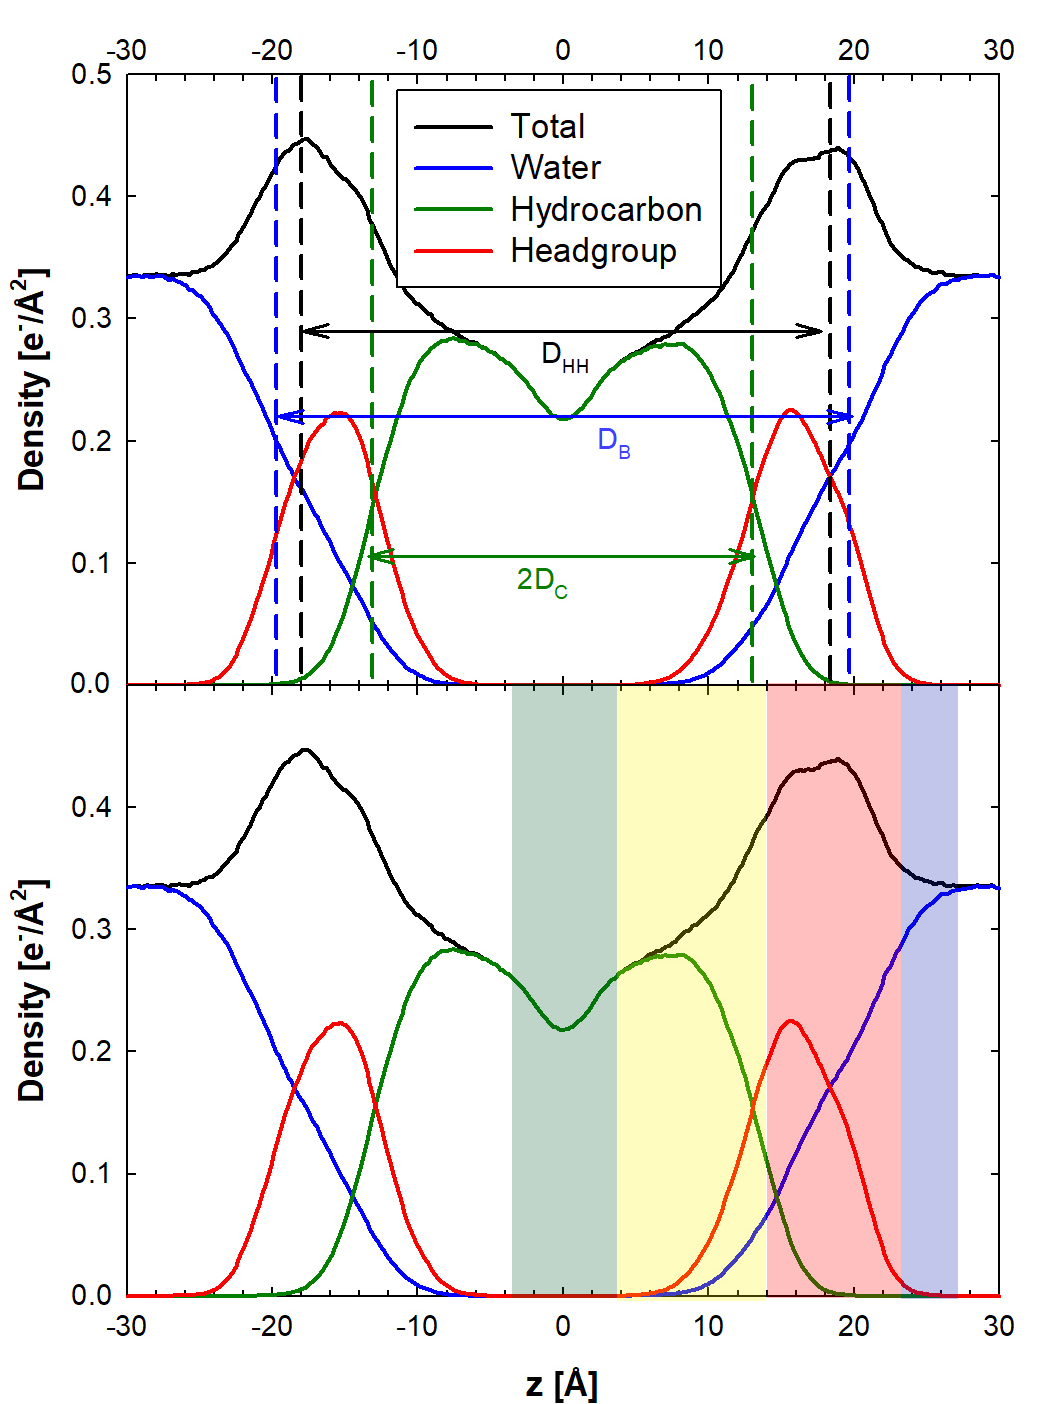
\includegraphics[width=\columnwidth]{figures/densityprofile.jpg}
	\caption{Transverse local electron density profiles for DMPC/cholesterol bilayer. Shown here are local density profiles for different molecular/atomic groups along the lipid normal for a fluid DMPC bilayer with 5\% cholesterol (top panel: different bilayer thickness definitions and bottom panel: four-region model with Regions 1, 2, 3, and 4 labeled as blue, red, yellow, and green, respectively). Data adapted from the simulation results of Boughter et al ~\cite{Boughter2016}.}
	\label{fig:density}
\end{minipage}
\end{figure}

\subsubsection{Transverse lateral stress profile}
\label{subsubsec:latstress}

The lateral stress profile in the transverse direction $P_{xy}(z)-P_z$ quantifies the equilibrium balance of stresses or forces acting between regions pointwise in a lipid bilayer.
This breakdown is only unambiguous for a model whose forces are themselves defined locally (for example, a continuum model whose forces act between infinitesimally separated points).
However, these ranged forces can be projected onto a continuum model, a transformation that requires the specification of a path (the contour) between non-local points.
As shown in ``Statistical mechanics of inhomogeneous fluids'' ~\cite{Society2014} by Schofield and Henderson, section IV, observables that can be cast as resulting from a global deformation of the system can be computed unambiguously from the profile, including curvature derivatives (see Sodt 2016 ~\cite{Sodt2016}, supplemental).
Care must be taken, however, to interpret local features of the profile qualitatively.
For example, it is appropriate to ask the question ``Does the model capture the qualitative structure of the competing forces in lipid bilayer assembly and stability?''

Despite its importance, however, the stress profile is often more difficult and expensive to calculate.
One means of calculating is through GROMACS-LS, a customized version of the MD package GROMACS.
GROMACS-LS can even calculate stress component profiles, including those arising from van der Waals and electrostatic interactions.
For more information about package and theory: \url{https://mdstress.org/} ~\cite{Torres-Sanchez2016,Torres-Sanchez2015,Vanegas2014a,Ollila2009}.
As an important verifying metric of force field development, the stress profile can be thoroughly compared with existing atomistic simulation studies.
There is no direct means of stress profile comparison with experiments, though as we will explain, properties calculated from the stress profile can be compared with experiment (Section~\ref{subsubsec:mechprops}).

\subsubsection{Bilayer thickness}
\label{subsubsec:thickness}
%\parbox{8.5cm}{\sloppy
%\begin{center}
%\begin{minipage}{\columnwidth}
%\centering
The membrane thickness is a structural metric that is consequently calculated from the density profile.
Three experimentally relevant definitions include (1) the Luzzati or total lipid thickness $D_B$, (2) the head-to-head distance $D_{HH}$, and (3) the hydrocarbon thickness $2D_C$.
The Luzzati thickness is relevant to neutron scattering, and is calculated as the distance between the two locations on each side of the bilayer where the water density drops to one half its bulk value.
This thickness metric in reality is based on the spatial profile of protiated and deuterated water, and is physically indicative of the degree of water penetration into the bilayer ~\cite{Poger2016}.
The head-to-head distance is relevant to x-ray scattering, and calculated as the distance between the two peaks in the electron density profile.
More simply, this can also be approximated as the distance between the maximal phosphate group densities in each leaflet, relevant to coarser lipid models ~\cite{Poger2016}.
The hydrocarbon thickness is also an important measure when comparing with transmembrane proteins and their length of surface exposure of the hydrophobic residues.
All of these thickness calculations can be indirectly compared with experiment, which for example can be obtained from neutron scattering--specifically, the difference between repeat spacing of lipid lamellae in water and the thickness of the water layer--or x-ray scattering--the same definition as in simulation ~\cite{Poger2016}.
Typical values for phospholipid bilayers in simulation and experiment are around 3 to 5 nm.
%\end{minipage}%
%\end{center}

\subsubsection{Area per lipid and NMR order parameter}
\label{subsubsec:aplnmr}
Two important structural parameters, complementary to one another, are (1) the area per lipid $a_l$, providing information about in-plane structure or lateral density, and (2) the deuterium NMR order parameter $S_{CD}$, providing information about out-of-plane structure.
Area per lipid and the deuterium NMR order parameter are shown schematically in Figure~\ref{fig:aplnmr}.

\begin{figure}[h]
\centering
\begin{minipage}[c]{\columnwidth}
\centering
	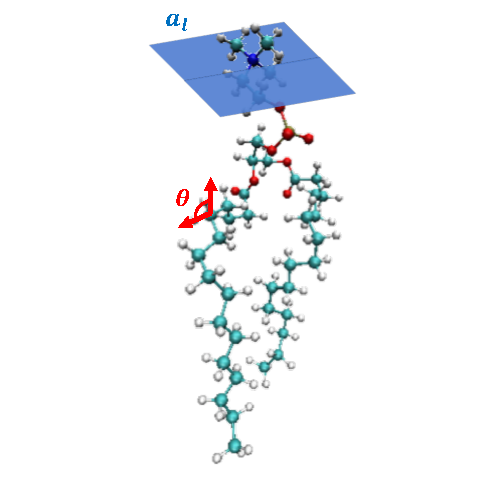
\includegraphics[width=\columnwidth]{figures/apl_nmr.pdf}
	\caption{Area per lipid and deuterium NMR order parameter definitions. Shown here for an all-atom DPPC phospholipid are the definitions of the area per lipid (blue plane) and an angle along one of the lipid acyl chains (red) used for the NMR order parameter calculation.}
	\label{fig:aplnmr}
\end{minipage}
\end{figure}

The area per lipid, or in-plane area occupied by a given lipid (illustrated in Figure~\ref{fig:aplnmr}), is a critical target in force field parameterization of lipid membranes ~\cite{Venable2015,Klauda2010d}.
In simulation, the area per lipid is typically calculated via

\begin{equation}\label{eq:5}
	%\label{e:partition}
	a_l=\frac{L_x L_y}{n}\
\end{equation}
where $n=N_l/2$ is the number of lipids per leaflet ~\cite{Poger2016}.
This equation assumes a lipid number symmetric bilayer with negligible undulations, such that the contour or membrane and projected or periodic box areas are roughly equal ~\cite{Venable2015,Klauda2010d}.
However, for larger membranes, undulations will lead to significant differences between the contour and projected areas.
Theoretically speaking, undulations will increase the ratio of contour area to the projected area, and this is specifically because the undulations reduce the projected areas ~\cite{Venable2015}.
The area per lipid is rigorously an intensive, or size-independent, quantity, so the appropriate steps should be taken to normalize for significant size effects when necessary before experimental comparison.
This may warrant simulation of different membrane sizes, extrapolating results to zero system size to allow for convergence of contour area to frame area and arriving at a size-independent metric ~\cite{Waheed2009}.
However, the area per lipid may not vary much across typical sizes of MD simulations, or even in experiments; thus, the simulation of different-sized membranes may not be a viable option.

In any event, care should be taken to ensure proper statistics and maximize precision.
Even at equilibrium, the area per lipid can fluctuate on a time scale of 10-100 ns ~\cite{Poger2016}, especially for complex bilayers and for those with many components.
For multicomponent membranes, the membrane should be partitioned into individual values for each lipid species.
Voronoi-based methods can be particularly useful for lipid mixtures in that they can partition the total bilayer area into individual area per lipid values for each species ~\cite{Poger2016}.
APL@Voro is a prominent Voronoi-based method for GROMACS trajectories, and supports projected area per lipid and bilayer thickness calculations for mixed lipid membranes and those including proteins ~\cite{Lukat2013}.
Partial molar areas can be determined, but this requires that a range of concentration ratios be simulated.
The area per lipid can be compared directly with other simulations; normalized size-independent metrics should be obtained where possible.
The value for double-tailed phospholipids is generally larger than single-chain hydrocarbons in systems like self-assembled monolayers (60 \AA$^2$/molecule versus 30-40 \AA$^2$/molecule).

The deuterium $P_2$ NMR order parameter describes the alignment of lipid constituent bonds with the global membrane normal, the $z$-direction for a bilayer assembled in the $xy$-plane, and will vary along the length of the lipid tail group chains and between liquid disordered and ordered or gel membranes.
For phospholipids, the NMR order parameter can also be used to validate the structure of the glycerol backbone and headgroup ~\cite{Botan2015}.
The metric is defined as:

\begin{equation}\label{eq:6}
	%\label{e:partition}
	S_{CD}=\frac{1}{2} \left<3\cos^2\theta-1 \right>.
\end{equation}
where $\theta$, illustrated in Figure~\ref{fig:aplnmr}, is the angle between a given carbon-deuterium bond along the lipid molecule and the global membrane normal and the brackets specify an ensemble average.
A value of 1 indicates perfect alignment of the chain with the global bilayer normal, while -0.5 indicates anti-alignment.
This metric, however, can be ambiguous.
For example, a value of zero can mean either that the lipids are isotropically disordered with respect to the bilayer normal, or that the lipids are perfectly oriented at a constant angle equal to the ``magic angle'' of 54.74$^{\circ}$ ~\cite{Poger2016}.

$NMRlipids$ (\url{https://www.nmrlipids.fi}) is a particularly new and multi-stage initiative launched by S. Ollila to determine the best possible lipid force fields on the basis of predicting NMR order parameters.
This initiative provides excellent guidance for simulation studies where correctly capturing these properties is essential.
Piggot et al. ~\cite{Piggot2017a} evaluates a host of tools for the calculation of NMR order parameters in simulation.
The study finds that, while existing tools are sufficient for saturated and all-atom lipids, some tools suffer from severe inaccuracies for unsaturated and united-atom ones ~\cite{Piggot2017a}.
Analysis tools like the NMRlipids united-atom approach and \textit{g\_lomepro} are two verifiable approaches for united-atom unsaturated lipids ~\cite{Piggot2017a}.
Computing error bars is tricky, but the $order\_parameters$ tool in LOOS ~\cite{Romo2009} offers one approach using sophisticated bootstrapping ~\cite{Romo2011}; LOOS is compatible with files generated from multiple MD packages, including AMBER, CHARMM, GROMACS, and NAMD.
For fluid membrane simulations, error bars can also be calculated under the assumption that each lipid molecule is a statistically independent entity ~\cite{Botan2015}.
Since the area per lipid and NMR order parameter of acyl chains are coupled, a similar magnitude of statistics ($\approx$10-100 ns) is required for $S_{CD}$ as well.
Calculated metrics can be compared with other simulations and directly with quadrupolar or dipolar NMR splitting experiments ~\cite{Ollila2016}.

Figure~\ref{fig:scd} shows typical order parameter profiles along the length of the lipid acyl chains for membranes of different lipid composition, and therefore different phase composition.
Increasing cholesterol composition transitions a DMPC bilayer from a liquid-disordered bilayer to a liquid-ordered one.
For a fluid phase bilayer from the top of the acyl chains to the bottom, values typically rise from about 0.17--0.20 to 0.20--0.22, then fall down to 0.10.
Averages across the entire chains are therefore typically around 0.17 ~\cite{Venable2015}.
Gel and liquid-ordered phase bilayer values are systematically larger across the acyl chains due to enhanced packing and ordering.

\begin{figure}
\centering
\begin{minipage}[c]{\columnwidth}
\centering
	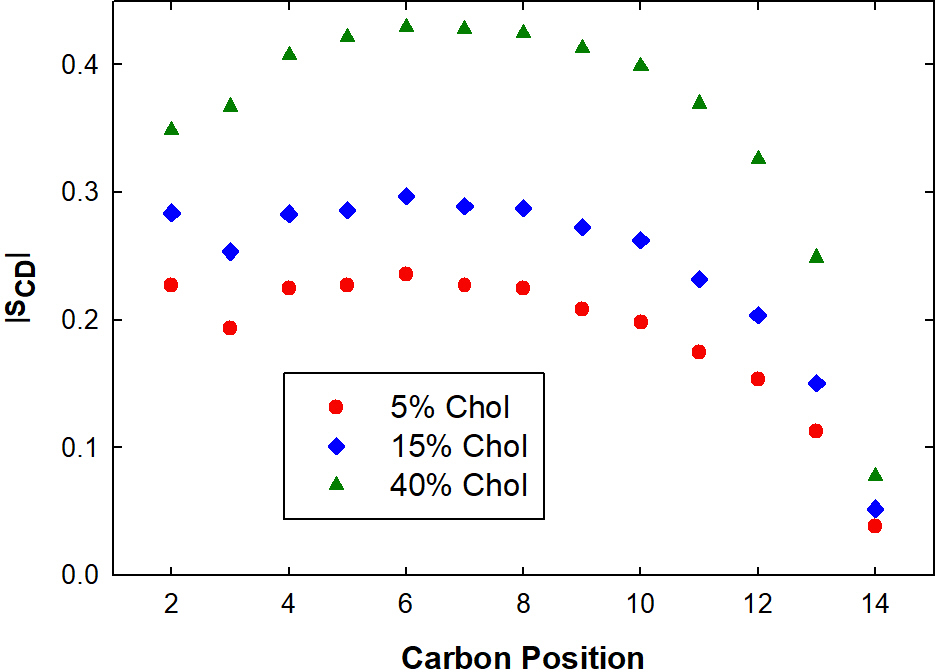
\includegraphics[width=\columnwidth]{figures/scd.jpg}
	\caption{Deuterium NMR order parameters for DMPC/cholesterol bilayers. Shown here are order parameter profiles along the lipid acyl chains for DMPC bilayers of increasing cholesterol composition, with values increasing from a $L_d$ (5\% cholesterol) to $L_o$ (40\% cholesterol) phase bilayer. Data adapted from the simulation results of Boughter et al ~\cite{Boughter2016}.}
	\label{fig:scd}
\end{minipage}
\end{figure}

While the area per lipid cannot be directly compared with experiments, due to the complications of lateral and transverse structure fluctuations, it can usually be inferred from a theoretical model that sometimes involves $S_{CD}$.
One example simply uses the lipid volume $V_L$ and the Luzzati thickness: $a_l=2V_L/D_B$.
This assumes, however, that the lipid volume can be estimated accurately ~\cite{Poger2016}.
Another approach uses the deuterium NMR order parameter: $a/chain=2V_{CH_2}/\big((1+2S)b_{cc}\big)$, where $a/chain$ is the area per tail group chain, of which there are two for double-tailed lipids, $V_{CH_2}$ is the volume of a $CH_2$ group, $S$ is the plateau value of $S_{CD}$--the maximum described above--and $b_{cc}$ is the projected C-C bond length along bilayer normal ~\cite{Nagle1993}.
Practically, these comparisons are difficult because $S_{CD}$ contains contributions from conformational disorder, local lipid tilting, and assorted collective motions ~\cite{Venable2015}.
While we do not recommend the above area per lipid models for the validation of lipid force fields, these models can at least be used for semiquantitative comparisons, e.g. comparisons of similar lipid components within the same phase (i.e. liquid ordered vs. disordered).

The best way to test validity of overall structural details of a bilayer is to compare with x-ray and neutron scattering form factors ~\cite{Ollila2016,Klauda2006a,Benz2005}.
These are direct measures for which experimental models can be used to estimate locations of functional groups in the membrane and the area per lipid.
The reported area per lipid in the literature is typically from these methods, but should be considered an indirect measure of this quantity.
The best comparison is made with the form factors, which are model independent ~\cite{Klauda2006a}.

\subsubsection{Lipid lateral diffusivity}
\label{subsubsec:latdiff}
The lipid lateral diffusivity $D_l$ is used to characterize lipid mobility, to gain insight into collective lipid motion timescales, and also potentially to discriminate between liquid crystalline and gel phase lipids.
The relevance of a diffusivity is predicated on the assumption of classical in-plane diffusion; however, depending on the system of interest, lipid lateral subdiffusion may be relevant (see Section~\ref{subsubsec:dynamicalnuances} for more information).
As such, the diffusivity can be determined from the slope of the average lipid mean-squared displacement (MSD) plotted against lag time, equal to $4D_l$ for 2D diffusion (\url{https://github.com/ejmaginn/TransportCheckList}).

In the MSD calculation, the user should be careful of artifacts due to lipid molecules partially or fully jumping across periodic boxes; periodicity can be accounted for by reimaging where appropriate.
For a homogeneous, single-component membrane, averages are normally taken over all lipids.
Results typically fall around $\mathcal{O}$($10^{-8}$ to $10^{-7}$ $cm^2/s$).
Simulation results can vary significantly with the force field, system size, truncation scheme for long-range interactions, time step, and non-bonded interaction pair list update frequency ~\cite{Poger2016}.
Venable et al. recommends that, when reporting and comparing with other simulations, the system size in particular should be noted and accounted for.
Given the hydrodynamic theory, the lateral and transverse dimensions would be even more explicit, and ideally, studies should report extrapolated infinite size values with a confidence interval ~\cite{Venable2017}.
The hydrodynamic theoretical framework has been extensively validated by V\"ogele and Hummer, who conducted MD simulations with up to $10^8$ coarse-grained particles in half-micron-sized boxes ~\cite{Vogele2018}.
Based on this recent work on size effects on lipid diffusivity, the \textit{memdiff} repository and package from the Hummer group (\url{https://github.com/bio-phys/memdiff}) provides Python implementations of finite-size diffusivity corrections and example applications.
Results can be indirectly compared with experiment.
Experimental estimates can generally vary over three orders of magnitude, due to a number of reasons ~\cite{Poger2016}.
For more details, see Section~\ref{subsubsec:dynamicalnuances}.

\subsubsection{Mechanical/elastic properties}
\label{subsubsec:mechprops}
Mechanical properties for membranes can be calculated from a number of techniques that can be broadly classified by (1) equilibrium fluctuations, (2) stress profile, and (3) biased/active deformations.
We discuss the merits of each umbrella of approaches in general terms in Section~\ref{subsubsec:mecheval}.
In this section, we merely attempt to recommend the best technique(s) to calculate a given property.
These mechanical properties include: (1) lateral tension, (2) area compressibility modulus, (3) bending modulus, (4) monolayer spontaneous curvature, (5) Gaussian curvature modulus, and (6) line tension.

(1) Calculation of the lateral tension $\gamma$ from a membrane simulation is a way to calculate the variable conjugate to the membrane [contour] area in canonical simulations, and in tension control, a way to directly confirm the simulation controls for the intended ensemble.
In model development, the tension is a parameter probed to capture the correct area per lipid, which should ideally occur at zero tension ~\cite{Zgorski2016}.
The tension is related to the zeroth moment of the stress profile, and can be easily approximated with the Kirkwood-Buff equation Equation~\ref{eq:1} above.

(2) The area compressibility modulus $K_A$ determines a membrane's ability to compress and expand, and is another important property in force field parameterization ~\cite{Venable2015}.
We recommend calculating $K_A$ based on area fluctuations in the tensionless ensemble:

\begin{equation}\label{eq:7}
	%\label{e:partition}
	K_A^{app} = \frac{k_BTA_p}{\sigma_{A_p}^2}\
\end{equation}
where $K_A^{app}$ is the apparent area compressibility modulus based on the fluctuations in projected area $A_p=L_x L_y$.
This equation is fairly simple, but involves two major nuances.
The first is that the calculation may take 100 ns to converge ~\cite{Venable2015}, if not longer.
The second is that this is an apparent value based on size-dependent projected area fluctuations, and is not the end point for characterizing the intensive, size-independent in-plane compressibility.
The recommended correction to deconvolute expansion-compression modes from undulatory modes is to simulate multiple membrane sizes and extrapolate the results to zero system size, where undulations no longer exist ~\cite{Waheed2009}.
At smaller simulated system sizes, the result of not accounting for undulatory contributions can be negligible ($\sim$5-10\% correction with experiment), but becomes substantial and must be corrected for larger system sizes (where they can be $\sim$50\% larger than experimental results)  ~\cite{Waheed2009,Venable2015}.
Results typically vary between 100 and 400 mN/m ~\cite{Venable2015}, and are often compared with micropipette aspiration experiments ~\cite{Rawicz2000}.
Results can also be compared with predictions from polymer brush theories, where $K_A$ is sometimes related to the oil-water interfacial tension $\gamma^{o/w}$--for example, $K_A = 6 \gamma^{o/w}$  ~\cite{Rawicz2000}.

(3) The bending modulus (bending rigidity/constant) $\kappa$ determines the ability of the membrane to bend.
The undulation spectrum method ~\cite{Goetz1999,Lindahl2000} is the traditional and well-established way to calculate $\kappa$.
On the basis that at large enough scales, a membrane behaves as a two-dimensional surface, the free energy per lipid can be expanded in terms of the area per lipid and mean and Gaussian curvatures $H$ and $K_G$ respectively ~\cite{Safran1994}.
In the absence of external stresses, a membrane minimizes its free energy with respect to area--i.e. it is tensionless--and shape, i.e. curvature, fluctuations are more accessible than expansion-compression or area compressibility fluctuations.

Canham and Helfrich developed a membrane Hamiltonian on this phenomenological basis, that a membrane has a preferred morphology dictated by its spontaneous curvature $C_0$ and has deviations from that preferred curvature ~\cite{Canham1970b,Helfrich1973a}, resulting in:

\begin{equation}\label{eq:8}
	\mathcal{H} = \int dS \Big[\frac{\kappa}{2}\ (2H-C_0)^2+\kappa_G K_G\Big]
\end{equation}
where $H\equiv(c_x+c_y)/2$, $c_x$ and $c_y$ are the principal curvatures, $\kappa_G$ is the Gaussian curvature modulus, and $K_G\equiv c_x c_y$.
This integral is performed over the entire surface of the membrane.
The integral over the Gaussian curvature term depends on the membrane topology and boundary, and does not contribute to the membrane energetics when topology and boundary do not change--i.e. when there are no membrane fission/fusion events, no pores/pre-pores, etc.
In this definition, $\kappa$ is the bare bending modulus, a ``true bilayer property'' and enthalpic/elastic quantity that represents a spring constant for curvature deformations.

For small deformations of a bilayer of zero spontaneous curvature ($C_0=0$), the first term of the integral is often presented in terms of the Monge gauge, with the surface described with respect to the $xy$-plane at $z = 0$ ~\cite{Safran1994}:

\begin{equation}\label{eq:9}
	\mathcal{H} = \int dxdy \Big[\frac{\kappa}{2}\ \big(\nabla^2 h(x,y)\big)^2\Big]
\end{equation}
where $h$ is the membrane height function and $x$ and $y$, as before, are the in-plane directions of the membrane.
By introducing a Fourier representation for $h$ and applying the equipartition theorem, one can derive the height-height undulation spectrum ~\cite{Brown2008}.
The spectrum describes the height-height correlations $\left|h_q\right|^2$ of the membrane continuum shape, and for a tensionless membrane, the large wavelength/small wavevector ($q$) behavior follows an inverse fourth power relation with a constant of proportionality that contains the bending modulus  ~\cite{Goetz1999,Lindahl2000}:

\begin{equation}\label{eq:10}
	\left< \left|h_q \right|^2 \right> = \frac{k_BT}{\kappa q^4}\
\end{equation}
The undulation spectrum method, however, must be used over ``mesoscopic'' length scales, approximately ten times the bilayer thickness, or about 50 nm / 5000 lipids, that are out of reach for AA and most CG simulations.
If simulations are too small, deviations to the undulation spectrum will result from individual lipid tilting (below ten thicknesses) and protrusions (below three thicknesses) ~\cite{Venable2015}.
Also, there will simply not be a large enough range of wave vector magnitudes to fit the spectrum and obtain a bending modulus estimate.

For this reason, we recommend the lipid director field spectrum approach ~\cite{Watson2012a,Venable2015}, which analyzes thermal fluctuations of lipid orientation via a director vector field $\hat{n}_q$, the vector from a lipid's head to its tail.
Specifically, the longitudinal component of the director field $\hat{n}_q^{||}$ relates to the macroscopic bending modulus through an inverse second power relation in the wave vector:

\begin{equation}\label{eq:11}
	%\label{e:partition}
	\left< \left|\hat{n}_q^{||} \right| \right> = \frac{k_BT}{\kappa q^2}\ \quad (recommended \: over \: Equation~\ref{eq:10})
\end{equation}
The lipid director field spectrum method works well for ``modestly sized'' membranes, down to approximately three bilayer thicknesses ($\approx$12-15 nm); AA simulations of 648 lipids have been shown to be well converged.
This general approach also provides a route to calculating bilayer tilt and twist moduli.
Both the undulation and lipid director field spectrum approaches will take at least 100 ns to converge  ~\cite{Venable2015}.

Equations ~\ref{eq:10} and ~\ref{eq:11} above relate membrane fluctuations to the bending modulus.
It is important to note that the $\kappa$ resulting from these methods is actually an apparent/effective bending modulus, a free energetic quantity incorporating the effects of finite size and thermal fluctuations.
The effective bending modulus is not a material property, and can be understood as a renormalization/correction from the bare value as first introduced by Peliti and Leibler.
It is dependent on system size, and decreases at larger wavelengths $\lambda$ as $\kappa(\lambda) = \kappa _0 - 3k_BT/4\pi ln(\lambda a)$, where $\kappa_0$ is the bare modulus and $a$ is some constant  ~\cite{Peliti1985}.
The determination of the appropriate size renormalization is somewhat ambiguous, but the length scale of the relevant experimental system can be used as a guide.
Furthermore, these techniques are only applicable in the small deformation/low curvature limit--i.e. in the absence of an external bending force).
The bare bending modulus is a size-independent quantity applicable at larger deformations/higher curvatures where ground state energies are dominant and fluctuation effects are negligible, and therefore may be more experimentally relevant.
Several, more user-intensive approaches have recently been introduced to directly measure the bare bending modulus ~\cite{Diggins2013,Hu2012a,Harmandaris2006a,DenOtter2003}; for more information, the interested reader is directed to those studies.

Bending modulus results typically vary between 10 and 40 $k_BT$ ~\cite{Venable2015}, and can be compared with a host of experimental techniques, including flicker spectroscopy and micropipette aspiration.
See Section~\ref{subsubsec:mecheval} for more details.
For more information on experimental and simulation approaches to calculating the bending modulus across various force fields, and particularly the inconsistencies in results, we direct the interested reader to Bochicchio and Monticelli ~\cite{Bochicchio2016}.
Results can also be compared with polymer brush theory, which relates $\kappa$ to $K_A$ and the bilayer hydrophobic thickness $h_{phob}$ via $\kappa = K_Ah_{phob}^2/24$ ~\cite{Rawicz2000}.
We do not recommend using polymer brush theory to obtain and report bending moduli, but recommend it as a point of comparison with bending moduli calculated from the techniques recommended above.

(4) While lipid bilayers, both planar and vesicular, have a net zero bilayer spontaneous curvature $C_0$, their monolayers individually may have a propensity to curve.
This propensity is quantified by the monolayer spontaneous curvature $c_0$, and is defined to be positive for a lipid that forms micelles and negative for one that forms inverted micelles ~\cite{Venable2015}.
Together with the monolayer bending modulus $\kappa_m$, $c_0$ is related to the first moment of the stress profile, integrated from the bilayer midplane to the upper edge of the simulation cell  ~\cite{Safran1994}:

\begin{equation}\label{eq:12}
	%\label{e:partition}
	\kappa_m c_0 = \int_{0}^{L_z/2} z[P_{xy}(z) - P_z]dz
\end{equation}
Thus, if $\kappa_m$ is known, then $c_0$ can be quantified.
$\kappa_m$ is predicted by elastic theory to be one half the bilayer value $\kappa$.
Monolayer spontaneous curvatures are typically calculated indirectly in experiment from studies in the completely different inverted hexagonal $H_{II}$ phase, where lipid monolayers are assembled in long, hexagonally-arranged water-filled tubes ~\cite{Gruner1986}.
Results are then extrapolated to the lamellar phase.
This is hard to study for lipids like DPPC that are more cylindrical in shape, but easier for those like dioleoylphosphatidylethanolamine (DOPE) that are more like inverted truncated cones due to acyl chain unsaturation ~\cite{Venable2015,Israelachvili2011}.

(5) The Gaussian curvature modulus $\kappa_G$ describes the propensity of the membrane to change topology, and is especially important for fission and fusion events ~\cite{Hu2012a}.
In general, even simulation methods for calculating $\kappa_G$ are controversial.
The difficulty in calculating $\kappa_G$ lies in controlling topology and boundary behaviors in which Gaussian curvature plays a role ~\cite{Hu2012a}.
The stress profile approach, specifically involving the second moment, is not reliable here  ~\cite{Hu2012a,Hu2013}.
We recommend the patch closure method, which has shown promise in preliminary work ~\cite{Hu2012a}.
Experimental analysis of the temperature dependence of the cubic to inverse hexagonal transition for N-monomethylated DOPE ~\cite{Siegel2008} is one of the few hints, with $\kappa_G / \kappa = -0.927$. %$\frac{\kappa_G}{\kappa}=-0.927$.  
Elasticity theories do offer predictions, for example, the simple approximation $\kappa_G \approx -\kappa$  ~\cite{Deserno2009,Hu2012a,Ramakrishnan2014c}.

(6) A line tension or edge energy $\Gamma$ is an energy per unit length that can describe lipid phase segregation and hole formation.
Specifically for pores--hydrophilic holes, where lipids splay to connect the two leaflets--the line tension can be studied through simulation of a bilayer ``strip'' or ``half-connected bilayer,'' with exposed bilayer edges in one in-plane box dimension.
The bilayer is thus periodic in one lateral dimension and exposed in the other, resulting in lipid splaying and therefore a rim on both sides.
In this scenario, the line tension can be determined from the stress profile, specifically the lateral normal stresses.
If the strip is periodic in $y$ and non-periodic in $x$, then:

\begin{equation}\label{eq:13}
	%\label{e:partition}
	\Gamma = \frac{1}{2}\ L_x L_y (P_{xx} - P_{yy})
\end{equation}
and $P_{xx} = P_{zz}$ ~\cite{Tolpekina2004b}.
Typical values are around 35 to 50 pN in simulation ~\cite{Tolpekina2004b,Wohlert2006} and 5 to 30 pN in experiment ~\cite{Brochard-Wyarta2000,Moroz1996,Zhelev1993}, the latter of which are typically determined through dynamical pore closure studies.

\subsubsection{Leaflet-dependent properties}
\label{subsubsec:leafprops}
Lipid bilayers are made up of two molecularly-thick leaflets in a fluctuating membrane embedded in three dimensions.
Identifying which lipid is in which leaflet at any given time is useful for identifying the local bilayer midplane, and therefore a host of bilayer and individual monolayer properties.
While thickness, area per lipid, deuterium order parameter, and lipid lateral diffusivity calculations do not necessarily require leaflet identification, other metrics do. Leaflet identification and the relevant metrics are discussed in Section~\ref{subsubsec:leafid-props}.


%%%%%%%%%%%%%%%%%%%%%%%%%%%%%%%%%%%%%%%%%%%%%%%%%%%%%%%%%%%%

% This provides a checklist which
% - spans a full page
% - consists of multiple sub-checklists
% - exists on a separate page
% This style of checklist will be especially helpful if you want to encourage readers to print and use your checklist in practice, as they
% can easily print it without also printing other material from your manuscript. However, other styles of checklist are also possible (below).
\begin{Checklists*}[p!]

\begin{checklist}{1. Model Selection}
\textbf{Goal: set up lipid membrane model to accurately capture properties of interest in an efficient manner.}
\begin{itemize}
\item Lay out problem/phenomenon of interest, and establish whether or not molecular simulations are needed.
\item If molecular simulations are needed, determine:
	\begin{itemize}
	\item Available computing resources (cores, memory, storage, etc.)
	\item Desired lamellar membrane configuration (planar vs. vesicular). See Section~\ref{subsubsec:geometry} for details.
	\item Relevant length and time scales of the system of study (or, if possible, of an appropriate subsystem). See Sections~\ref{subsubsec:prodrun} and \ref{subsubsec:size} for a discussion.
	\item Primary properties of interest (structural, mechanical, thermodynamic, and/or dynamic)
	\item Required spatiotemporal resolution; desired membrane composition; relevance of ions
	\end{itemize}
\item Based on the above considerations, determine the optimal model in terms of accuracy and efficiency.
\end{itemize}
\end{checklist}

\begin{checklist}{2. Pre-Simulation Considerations / Selection of MD Settings}
\textbf{Goal: establish rational and physically-intuitive settings for the desired lipid membrane simulation.}
\begin{itemize}
\item Determine desired thermodynamic ensemble.
\item Given selected model and experimental correspondence, determine target temperature.
\item If relevant, determine pressure control settings.
\item Determine remaining settings necessary for MD configuration file.
\end{itemize}
\end{checklist}

\begin{checklist}{3. Preparation of Initial Configurations}
\textbf{Goal: build reasonable equilibrium starting structure for a lipid bilayer in a periodic simulation box.}
\begin{itemize}
\item From the desired membrane size and geometry, estimate the number of required lipids (Equations~\ref{eq:2} and \ref{eq:4a}).
\item Estimate the number of solvent molecules and full periodic box dimensions (Equations~\ref{eq:3} and \ref{eq:4b}).
\item Using the above estimates, proceed through to system setup. See Section~\ref{subsubsec:construction} for options.
\item Minimize (no dynamics) to remove bad site contacts.
\item Anneal from 0 K to target temperature.
\item Equilibration
	\begin{itemize}
	\item For a templated membrane, just equilibrate
	\item For membrane self-assembly, assemble, then equilibrate
	\end{itemize}
\item Qualitatively confirm equilibrium structure and quantitatively confirm equilibration of thermodynamic averages before a production run.
\item Rotate/re-center system as necessary.
\item Determine reasonable amount of sampling for production run. See Section~\ref{subsubsec:prodrun} for details.
\end{itemize}
\end{checklist}

\begin{checklist}{Simulation Production Run}
\end{checklist}

\begin{checklist}{4. Post-Simulation Considerations / Validation of Calculated Properties}
\textbf{Goal: comprehensively justify simulation procedure and model selection via rigorous production run analysis.}
\begin{itemize}
\item Calculate and validate bilayer structure via thickness, area per lipid, scattering form factors, and NMR order parameters.
\item Calculate and validate lipid lateral diffusivity, bilayer stress profile and mechanical properties as necessary.
\item If required, set up and run additional simulations (e.g. for more time, with external biases, etc.) for certain property determinations. Determine if leaflet identification is necessary for other metric calculations. Proceed as necessary.
\item For the relevant properties, assess model artifacts due to simplified composition/resolution, finite system size, and simulation time scale.
\end{itemize}
\end{checklist}

\end{Checklists*}

%%%%%%%%%%%%%%%%%%%%%%%%%%%%%%%%%%%%%%%%%%%%%%%%%%%%%%%%%%%%

\section{Rationale for checklist choices}
\label{sec:rationale}

In this section, we elaborate on items in the checklist. Where relevant, we include details on alternatives, compare different approaches, and provide physical and literature justification.

\subsection{Model selection}
\label{subsec:models4}
Efficiency is a major concern in virtually any lipid membrane simulation.
In the MD loop, the most expensive step involves the pairwise force evaluations, and therefore the number of particles in your system $N$ and the system density $\rho_{model} \propto 1/a_{model}^3$, where $a_{model}$ is the average spacing between sites in the model.
Exact simulation time $t_{sim}$ scalings depend on the force field, and can range from $N \rho_{model}$ for short-ranged/mean field types of force fields to $NlogN$ to $N^2$ for long-ranged/rigorous pairwise interactions.
The number of particles can be related to the system density $\rho_{model}$ and the system length scale $L$, which for a cubic box results in:

\begin{equation}\label{eq:14}
	%\label{e:partition}
	N = \left\{
        		\begin{array}{ll}
            		\rho_{model} L^3 & \quad (explicit \: solvent) \\
            		\rho_{model} L^2 & \quad (implicit \: solvent).
        		\end{array}
    	\right.
\end{equation}
This scaling incorporates the model resolution $\rho_{model}$ and system size $L$/nature of solvent, respectively.
Thus, for short-ranged interactions:

\begin{equation}\label{eq:15}
	%\label{e:partition}
	t_{sim} \propto \left\{
        		\begin{array}{ll}
            		\rho_{model}^2 L^3 & \quad (explicit \: solvent) \\
            		\rho_{model}^2 L^2 & \quad (implicit \: solvent)
        		\end{array}
    	\right.
\end{equation}
and for long-ranged:

\begin{equation}\label{eq:16}
	%\label{e:partition}
	t_{sim} \propto \left\{
       		 \begin{array}{ll}
            		\rho_{model}^2 L^6 & \quad (explicit \: solvent) \\
            		\rho_{model}^2 L^4 & \quad (implicit \: solvent).
        		\end{array}
    	\right.
\end{equation}

There is additionally a system size contribution, added to the geometric one, that accounts for sufficient sampling.
This accounts for the largest wavelength undulations that are the slowest degree of freedom, and scale as $L^3$ ~\cite{Watson2010a}.
This is based on the theory of Zilman and Granek, modeling the membrane structure factor based on its approximation as a thin structureless sheet in viscous fluid ~\cite{Zilman2002,Zilman1996}.
Thus, the overall scaling in system size can be from $L^5$ up to $L^9$, depending on the range of interactions and presence/absence of solvent.
In other words, at a minimum, an order of magnitude increase in membrane length scale leads to five order of magnitude increase in computational expense!
Coarser models may contribute to higher accessible time scales in two ways: (a) by increasing the time scale of the fastest vibrational mode (i.e. $t_{sim} \propto \Delta t_{model}$) and (b) by also inherently smoothening the free energy landscape, and therefore enhancing dynamics across it, e.g. via a simple scale factor.
Finally, computing resources and the specific MD package affect the range of possible parallelization schemes--for example, domain decomposition--and determine the intrinsic speed of your simulations.

\subsubsection{Survey of lipid membrane models}
\label{subsubsec:modelsurvey}
In general, there is a very diverse range of models that can be leveraged for simulations of lipid bilayer membranes.
An extensive summary of prominent lipid membrane force fields, along with the notable pros and cons of each, is presented in Table~\ref{tab:forcefields}.

Atomistic (all-atom, or AA) models are the ``gold standard,'' as is the case with MD simulations of most other systems.
The quality of AA MD simulations of lipid bilayers has improved dramatically since their initial development in the early 1990s ~\cite{Venable2015}.
AA models can have hundreds of atomic sites per lipid molecule.
United atom (UA) force fields remove hydrogen atoms for an increase in efficiency (factor of $\sim$2-3) ~\cite{Lyubartsev2016}, and are competitive with AA force fields in accuracy.
AA and UA can therefore easily reach the 100 ns time scale and 5 to 10 nm length scales  ~\cite{Smirnova2015}, but with the appropriate resources and GPU-enabled codes, microsecond timescales are attainable.
Well-validated force fields include CHARMM36 (AA) ~\cite{Klauda2010d}, Slipids (AA) ~\cite{Jambeck2012}, AMBER Lipid14 (AA) ~\cite{Dickson2014}, and GROMOS 54A7 (UA) ~\cite{Poger2010a}.

Alternatively, coarse-grained (CG) models are well-developed for the efficient, large-scale simulation of lipid membranes, often where the interest is in mechanical and qualitative behaviors and less in the quantitative and chemical detail.
That said, systematic CG models can still retain some level of chemical specificity like the types of lipids that they represent.
CG models can be bottom-up, parameterizing CG parameters with atomistic data; top-down, parameterizing to capture certain macroscopic quantities or qualitative phenomena; or a combination of the two.
CG models can easily reach 1000 ns (1 $\mu$s) time scales and $\sim$20 nm length scales  ~\cite{Smirnova2015}, but can go beyond this toward the 100 $\mu$s with the proper resources.
One of the best-known CG models for membranes is the Martini force field  ~\cite{Marrink2004,Marrink2007a}, which via a 4:1 heavy or non-hydrogen atom mapping reduces to about ten pseudoatom sites per lipid.

Because the aqueous solvent can contribute up to 90 percent of the force evaluations ~\cite{Arnarez2015}, implicit solvent (IS) simulations can be much more efficient and potentially advantageous.
Examples of IS CG models include the Dry Martini force field ~\cite{Arnarez2015}, the implicit solvent analog of (``wet'') Martini; the five-site model of Brannigan and Brown ~\cite{Brannigan2005b}; and the three-site model of Cooke, Kremer, and Deserno ~\cite{Cooke2005a}.
For proper dynamical correlations and conservation of momentum, CG models (particularly IS) are sometimes executed with a fluctuating hydrodynamics ~\cite{Zgorski2016,Wang2013} or dissipative particle dynamics (DPD) ~\cite{Deserno2009} thermostat.
These models extend the range of accessible scales even further to 100 $\mu$s and 100 nm  ~\cite{Smirnova2015}

All force fields listed above are based on simplifications for long-ranged electrostatics and van der Waals interactions.
Most lipid force fields have been parameterized using long-ranged electrostatics with Particle-Mesh Ewald (PME).
However, long-ranged van der Waals interactions have not been included in force field parameterization for the assembled bilayer.
Therefore, researchers must conform to the standard Lennard-Jones (LJ) cutoff scheme recommended for the force field.
In the future, lipid parameterization will include the use of PME for LJ interactions ~\cite{Leonard2018} to avoid this artificial cutoff dependence.

In Table~\ref{tab:forcefields}, we do not include polarizable force fields that can account for problems with molecules parameterized in water that may also enter the vastly different dielectric environment of the membrane, thereby more accurately capturing energies and partitioning.
Interestingly, the implicit inclusion of polarizability can improve predictions of cation binding affinity to phosphatidylcholine lipid bilayers.
Existing nonpolarizable MD force fields tend to overestimate phospholipid cation binding affinity ~\cite{Melcr2018}.
Melcr et al. found a significant improvement in the binding affinity of Na$^+$ and Ca$^{2+}$ ions to a POPC bilayer by implicitly including electronic polarization as a mean field correction to the lipid headgroup region, particularly for the nonpolarizable Lipid14 and CHARMM36 models ~\cite{Melcr2018}.
The model they develop captures experimentally measured structural parameters for an ion-free membrane, the response of the lipid headgroup structure to a strongly bound catonic amphiphile, and the binding affinities of Na$^+$ and Ca$^{2+}$, suggesting for Ca$^{2+}$ a more complex binding stoichiometry than those of simpler, nonpolarizable models ~\cite{Melcr2018}.
Polarizable models can therefore provide richer interpretation of NMR data, amongst other benefits ~\cite{Melcr2018}.
Otherwise, the dielectric permittivity in the membrane interior is generally low, and polarizability effects are thus minimal.
Furthermore, dipole relaxations can significantly slow down simulations, impacting efficiency and making polarizable force fields completely impractical for large-scale membrane simulation studies.
For more information on polarizable models, see the work of Melcr et al. as well as custom force fields like AMOEBA ~\cite{Ponder2010} and CHARMM Drude ~\cite{Vanommeslaeghe2015}.



\nopagebreak[4]
\onecolumn
\nopagebreak[4]
\begin{center}
\begin{longtable}[h]{| p{1in} | p{3.25in} | p{2.25in} |}
\caption{Lipid membrane force fields: a survey} \\
\hline
\label{tab:forcefields}
\textbf{Force field (FF)} & \textbf{Notable pros} & \textbf{Notable cons} \\
\hline
\endfirsthead
\textbf{\textit{Atomistic (AA)}} & \textbf{\textit{``Gold standard'': Full chemical detail of lipids and optimized against various experimental measures}} & \textbf{\textit{Expensive, and therefore impractical for many large-scale membrane applications; does not typically account for polarizability}} \\
\hline
CHARMM36 ~\cite{Klauda2010d} & \begin{minipage}[t]{\linewidth} \begin{itemize}[nosep,after=\strut] \item Accurately represents many key bilayer properties: area per lipid, volume per lipid, electronic density profile, structure factor \item Operable in tensionless state \item Useful for membranes with cholesterol and studies of flip-flop \item Most diverse of AA FF with sphingolipids, ceramides, glycolipids, etc. \item Accurate with variations in temperature and phase changes ~\cite{Khakbaz2018,Zhuang2016a} \item Compatible with CHARMM parameters for carbohydates, proteins, and nucleic acids ~\cite{Javanainen2016,Pluhackova2016} \item Used extensively with membrane proteins ~\cite{Javanainen2016} \item Implemented and available in a variety of conventional MD packages (CHARMM, NAMD, GROMACS, etc.) ~\cite{Lyubartsev2016} \item Compatible with \textit{CHARMM-GUI} \end{itemize} \end{minipage} & \begin{minipage}[t]{\linewidth} \begin{itemize}[nosep,after=\strut] \item Results currently dependent on cutoffs used for FF development (1-1.2 nm) \item Inaccurate dipole potential drop with fixed charge models \item Some inaccuracies with ion FF parameters \end{itemize} \end{minipage} \\
\hline
Slipids ~\cite{Jambeck2012,Jambeck2012b,Jambeck2013a} & \begin{minipage}[t]{\linewidth} \begin{itemize}[nosep,after=\strut] \item Captures experimental area per lipid, NMR order parameters and structure factors, and temperature dependencies thereof \item Able to reproduce structural properties of single- and double-component membranes without surface tension application \item Generally amenable to the $NPT$ ensemble \item Many lipid types, including sphingomyelin, cholesterol, and polyunsaturated lipids ~\cite{Ermilova2016} \item Compatible carbohydrate force field \item Parameterization of small molecules available ~\cite{Javanainen2016} \item Compatible with AMBER FF and its amino acid and drug-related compounds ~\cite{Lyubartsev2016} \end{itemize} \end{minipage} & \begin{minipage}[t]{\linewidth} \begin{itemize}[nosep,after=\strut] \item Optimization approach similar to CHARMM36, yet not necessarily superior to it \item Less diverse options in lipids compared to CHARMM36 \end{itemize} \end{minipage} \\
\hline
Lipid14 ~\cite{Dickson2014} & \begin{minipage}[t]{\linewidth} \begin{itemize}[nosep,after=\strut] \item Captures experimental area per lipid, volume per lipid, lipid thickness, NMR order parameters, scattering data, and lateral lipid diffusion \item Allows tensionless $NPT$ simulations of a number of lipid types and cholesterol ~\cite{Javanainen2016} \item Compatible with AMBER protein, nucleic acid, carbohydrate, and small molecule force fields ~\cite{Lyubartsev2016} \end{itemize} \end{minipage} & \begin{minipage}[t]{\linewidth} \begin{itemize}[nosep,after=\strut] \item Limited to a few lipids and less diverse compared to Slipids and CHARMM36 (saturated, monounsaturated, PC and PE lipids) \end{itemize} \end{minipage} \\
\hline
OPLS-AA ~\cite{Maciejewski2014} & \begin{minipage}[t]{\linewidth} \begin{itemize}[nosep,after=\strut] \item Captures experimental area per lipid and X-ray form factors \item Captures deuterium order parameters overall \item Compatible with OPLS for organic liquid molecules, proteins, nucleic acids, carbohydrates, and drug molecules ~\cite{Lyubartsev2016} \end{itemize} \end{minipage} & \begin{minipage}[t]{\linewidth} \begin{itemize}[nosep,after=\strut] \item Limited range of lipids covered (lowest for AA lipid FFs) \item Discrepancies with experimental deuterium order parameters for first carbon along acyl chains ~\cite{Lyubartsev2016} \end{itemize} \end{minipage} \\
\hline
\textbf{\textit{United Atom (UA)}} & \textbf{\textit{Detailed, and yet $\sim$2-3 times more efficient than AA simulations without explicitly including non-polar hydrogens}} & \textbf{\textit{Still expensive and impractical for large-scale membrane simulations; does not account for polarizability}} \\
\hline
GROMOS (e.g. 45A3 ~\cite{Chandrasekhar2003}, 53A ~\cite{Oostenbrink2004}, 54A ~\cite{Poger2010a}, Berger modification ~\cite{Berger1997b}) & \begin{minipage}[t]{\linewidth} \begin{itemize}[nosep,after=\strut] \item Focus on capturing enthalpies and free energies of solvation \item Diverse options of lipids similar to the level of diversity in CHARMM36 \item Compatible with GROMOS parameter sets for proteins, carbohydrates, and nucleic acids \item Parameterization available for small molecules (e.g. Automated Topology Builder ~\cite{Malde2011}) ~\cite{Javanainen2016,Lyubartsev2016} \end{itemize} \end{minipage} & \begin{minipage}[t]{\linewidth} \begin{itemize}[nosep,after=\strut] \item Problems in representing proper gel phase of bilayer at temperatures below melting point ~\cite{Lyubartsev2016} \end{itemize} \end{minipage} \\
\hline
\textbf{\textit{Explicit solvent coarse-grained (CG)}} & \textbf{\textit{At least an order of magnitude more efficient than AA and UA, and can therefore access larger length and time scales, specifically larger-scale membranes and phenomena like undulations, self-assembly, phase transformations, phase coexistence, and interactions with macromolecules and nanoscale compounds}} & \textbf{\textit{Less accurate; sometimes semiquantitative or just qualitative; sometimes distorted dynamics due to smoothened free energy landscape}} \\
\hline
Martini ~\cite{Marrink2007a,Marrink2004} & \begin{minipage}[t]{\linewidth} \begin{itemize}[nosep,after=\strut] \item Combined bottom-up and top-down model, using atomistically-derived bonded parameters and nonbonded parameters that capture enthalpies, free energies of solvation \item Repository for a host of lipid types similar to CHARMM36 level of diversity \item Compatible with Martini protein and peptide, carbohydrate, and nucleic acid models \item Lots of tools available on website ~\cite{Lyubartsev2016,Javanainen2016} \item Broad range of applications \item Hydrodynamics thermostats in development ~\cite{Zgorski2016} \item Compatible with \textit{CHARMM-GUI} ~\cite{Qi2015a} \end{itemize} \end{minipage} & \begin{minipage}[t]{\linewidth} \begin{itemize}[nosep,after=\strut] \item No major repulsive interactions/mostly soft attractive \item Molecular polarity can be difficult to capture \item Aphysical water model (4:1 molecule mapping), the first of which freezes at standard temperatures (must incorporate ``antifreeze'' particles) \item Later solvent models capture polarity and polarizability ~\cite{Yesylevskyy2010}, but with drop in efficiency \item Interactions are shifted and truncated, and therefore short-ranged ~\cite{Lyubartsev2016} \end{itemize} \end{minipage} \\
\hline
ELBA ~\cite{Orsi2011} & \begin{minipage}[t]{\linewidth} \begin{itemize}[nosep,after=\strut] \item Good for electrostatics (includes dipoles into both lipid molecules and water beads) ~\cite{Javanainen2016} \end{itemize} \end{minipage} & \begin{minipage}[t]{\linewidth} \begin{itemize}[nosep,after=\strut] \item Limited lipid types available ~\cite{Javanainen2016} \end{itemize} \end{minipage} \\
\hline
\textbf{\textit{Implicit solvent coarse-grained (IS CG)}} & \textbf{\textit{$\mathcal{O}(10^0-10^3)$ times more efficient than AA and UA, and can therefore access the largest length and time scales of all particle-based simulations; useful for studying phenomena like undulations, self-assembly, phase transformations, phase coexistence, and interactions with macromolecules and nanoscale compounds}} & \textbf{\textit{Less accurate; sometimes semiquantitative or just qualitative; fluid phase may be unstable or require stabilization; some have problems with self-assembly ~\cite{Cooke2005d}; further distorted dynamics due to smoothened free energy landscape and lack of solvent}} \\
\hline
Dry Martini ~\cite{Arnarez2015} & \begin{minipage}[t]{\linewidth} \begin{itemize}[nosep,after=\strut] \item Up to 10$^3$ times faster than atomistic models ~\cite{Arnarez2015} \item Combined bottom-up and top-down model \item Captures experimental area per lipid, bilayer thickness, bending modulus, and liquid order-disorder coexistence \item Significant speedup permitting study of multicomponent, large-scale membranes \item Host of lipid types \item Compatible with other molecular models and broad range of applications \item Hydrodynamics thermostats in development with minimal computational overhead (still $\sim$4 times more efficient than explicit solvent ``wet'' Martini ~\cite{Lyubartsev2016,Arnarez2015,Zgorski2016}) \item Compatible with \textit{CHARMM-GUI} ~\cite{Qi2015a} \end{itemize} \end{minipage} & \begin{minipage}[t]{\linewidth} \begin{itemize}[nosep,after=\strut] \item No major repulsive interactions/mostly soft attractive \item Molecular polarity can be difficult to capture \item No explicit water dynamics and physics in general \item Difficulty in capturing solvent-mediated effects \item Energetically-dominated/inaccurate energy-entropy breakdown \end{itemize} \end{minipage} \\
\hline
PLUM ~\cite{Bereau2009,Wang2009c,Bereau2014a} & \begin{minipage}[t]{\linewidth} \begin{itemize}[nosep,after=\strut] \item Contains parameters for lipids and proteins \item Describes protein folding ~\cite{Javanainen2016} \end{itemize} \end{minipage} & \begin{minipage}[t]{\linewidth} \begin{itemize}[nosep,after=\strut] \item Limited to a few lipids \end{itemize} \end{minipage} \\
\hline
Models of Izvekov and Voth ~\cite{Izvekov2005,Srivastava2013} & \begin{minipage}[t]{\linewidth} \begin{itemize}[nosep,after=\strut] \item Models available at various resolutions \item Efficient \item Multiscale coarse-graining (MS-CG) method bottom-up, and therefore preserves certain microscopic properties of system \item Coarse-graining method incorporates both energetic and entropic driving forces \item Reproduces fluid lipid bilayer with accurate structural and elastic properties ~\cite{Izvekov2005} \end{itemize} \end{minipage} & \begin{minipage}[t]{\linewidth} \begin{itemize}[nosep,after=\strut] \item Limited to a few lipids \end{itemize} \end{minipage} \\
\hline
Model of Brannigan and Brown ~\cite{Brannigan2005b} & \begin{minipage}[t]{\linewidth} \begin{itemize}[nosep,after=\strut] \item Efficient (one head bead, one interface bead, three tail beads, and implicit solvent) \item Relative to Cooke model, treats hydrocarbon groups at membrane interface differently from those at membrane core \item Self-assembles \item Experimentally reasonable fluid and elastic properties \item Tunable properties ~\cite{Brannigan2005b,Brannigan2006} \end{itemize} \end{minipage} & \begin{minipage}[t]{\linewidth} \begin{itemize}[nosep,after=\strut] \item Generic/unclear chemical mapping \item Semiquantitative results \item General overprediction of experimental and explicit solvent simulation bending moduli ~\cite{Bochicchio2016} \end{itemize} \end{minipage} \\
\hline
Model of Cooke, Kremer, and Deserno ~\cite{Cooke2005d} & \begin{minipage}[t]{\linewidth} \begin{itemize}[nosep,after=\strut] \item Very efficient (one head bead, two tail beads, and implicit solvent) \item Competitive with and up to $\sim$5 times faster than DPD simulations of similar resolution \item Displays correct large-scale elastic behavior \item Tunable physical properties \item Stable fluid and gel phases \item Self-assembles \item Can model mixed-lipid systems ~\cite{Cooke2005d} \item Compatible with hydrodynamics thermostats ~\cite{Wang2013} \end{itemize} \end{minipage} & \begin{minipage}[t]{\linewidth} \begin{itemize}[nosep,after=\strut] \item Generic/unclear chemical mapping \item Treats hydrocarbon groups at membrane interface the same as those at membrane core ~\cite{Brannigan2006} \item Semiquantitative results \item General underprediction of experimental and explicit solvent simulation bending moduli ~\cite{Bochicchio2016} \end{itemize} \end{minipage} \\
\hline
\end{longtable}
\end{center}
\nopagebreak[4]
\twocolumn
\nopagebreak[4]

For lipid membranes, there is also an extensive subcommunity that uses continuum mechanical theory and field-theoretic simulations that are sometimes in fact the preferred approach at larger length scales (100 nm to 100 $\mu$m) due to their efficiency ~\cite{Smirnova2015,Brown2008,Sapp2014}.
These approaches are predicated on the above continuum theoretical framework, and can be performed on the basis of energy minimization of a continuum Hamiltonian and dynamical evolution of a continuum equation of motion for near-flat membranes; a surface-of-evolution approach for axisymmetric membrane shapes or deformations; direct numerical minimization for both axisymmetric and non-axisymmetric shapes; Fourier Space Brownian Dynamics, which has been applied to protein mobility on membranes and the effect of cytoskeletal pinning on membrane dynamics ~\cite{Brown2008,Brannigan2006,Lin2005,Lin2004}; dynamically triangulated Monte Carlo for irregular, fluctuating membranes; and Monte Carlo on a lattice  ~\cite{Brannigan2006d,Ramakrishnan2014c}.
It is often crucial to compare with these techniques wherever possible.
If some of the above conditions motivating the use of molecular simulations are not met (Section~\ref{sec:intro}), it is useful to evaluate whether or not a continuum approach would be better.

It should be evident from the thermodynamic and statistical mechanical framework above that there are some crucial considerations for any lipid membrane model, regardless of resolution, including: (1) composition, (2) other thermodynamic constraints, (3) model size, and (4) model geometry.

\subsubsection{Composition}
\label{subsubsec:composition}

It is generally important to consider the chemical mapping of the model to the real system, especially for multicomponent membranes.
The desired heterogeneity and particular lipids may determine the model one ultimately chooses.
In early simulations of lipid membranes for both AA/UA and CG resolutions, the canonical lipid of choice was DPPC (dipalmitoylphosphatidylcholine), with two fully saturated 16-carbon chains in water.
DPPC is a common choice for vesicle experiments and is a major component of pulmonary surfactant.
PC in general is the most abundant head group in mammalian and yeast membranes ~\cite{VanMeer2008,Sampaio2011}.
DPPC/water is typically the system for which new force fields are first tested.
However, DPPC is sometimes not preferred in experiments, due to its high melting point from the gel to liquid-crystalline state.
A more relevant lipid is the 14-carbon chain DMPC or one that has a chain with a single double bond or unsaturation like POPC.

The recent progression in the field is to go beyond single-component membranes toward more realistic membrane mixtures ~\cite{Khakbaz2015}.
For multicomponent membranes, there is a well-established body of literature.
For phase coexistence studies, typical model experiments consists of a ternary mixture of cholesterol and both saturated and unsaturated lipids ~\cite{Berkowitz2009}, but more biologically-relevant studies include greater than three lipid types ~\cite{Khakbaz2015}.
In fact, for biologically-relevant simulations, we advise caution in the selection and relative composition of lipids in the membrane model.
While there are good guidelines for the contributions of major lipid head and tail groups to biological membranes via major progress in lipidomics ~\cite{VanMeer2008,Sampaio2011}, composition can potentially vary across different domains and even between the two leaflets ~\cite{Ing??lfsson2014}, and the best choice for a given model will depend highly on the analogous experimental system.
The development of biologically-relevant membranes is at the forefront of the field for AA and CG models  ~\cite{Khakbaz2015,Monje-Galvan2015}, and in probing biological processes, one must ensure a membrane of the appropriate phase and composition, as proteins may function best in their native lipid environment.

When simulating a lipid membrane, ions may be required to match conditions in experiment and/or model systems.
The ion concentration in a typical human environment is 0.15 M ~\cite{Lodish2000}.
If a membrane has negatively-charged lipids, then to maintain electroneutrality small counter ions are needed such as K$^+$ or Na$^+$.

\subsubsection{Other thermodynamic constraints}
\label{subsubsec:constraints}
Given a membrane's composition, the thermodynamic constraints of temperature and tension or area will largely determine phase behavior.
As discussed above, simulations are sometimes amenable to different constraints from experiments (Section~\ref{subsec:presim3}), but the appropriate experimental conditions can be achieved in a corresponding simulation ensemble.
It is worth noting that certain models, both AA and CG alike, sometimes experience difficulty in capturing phase transition temperatures and even entire phases--for example, subgel and ripple for Martini ~\cite{Rodgers2012,Pluhackova2016}.

\subsubsection{Model size}
\label{subsubsec:size}
Whether or not the membrane physically reflects the experimental setup also depends largely on the dimensions of the model.
It has been shown for membranes that finite size effects can play a significant role for thermodynamic, especially mechanical, and dynamical properties ~\cite{Castro-Roman2006,Waheed2009,Venable2015,Venable2017}.
This refers not only to the in-plane dimensions, but also for the out-of-plane one; despite the quasi-two-dimensional structure of membranes and two-dimensional approximation at larger length scales, hydrodynamic theoretical models for periodic systems have shown that the thickness of the water layer(s) matter as well in convergence to macroscopic system dynamics ~\cite{Venable2017}.
In determining the model dimensions, one should search for the emergent length scales in the experimental system that can serve as the periodicity length scales in the simulation.
For biological membranes, there is experimental evidence to show that an appropriate in-plane length scale is around 150-500 nm.
This is set by the cortical cytoskeletal mesh, which pins membrane proteins and therefore constrains lipid motion per the anchored protein picket model ~\cite{Ritchie2003,Morone2006}.
This is too large for most molecular simulations, but if a highly resolved picture of biological membranes is still desired, different subsystems can be simulated.
If you do not simulate the relevant size of the overall experimental system or a relevant subsystem, then you need to be able to normalize your results with respect to the difference in sizes.

\subsubsection{Model geometry}
\label{subsubsec:geometry}
In many cases, experimental vesicles are modeled with planar bilayer simulations.
This may raise questions about the meaning of the results, as vesicular membranes are the result of a balance of positive strain on the outer leaflet and negative strain on the inner leaflet, while planar membranes have on average zero strain on each leaflet.
Furthermore, vesicles often have a different number of outer and inner leaflet lipids.
Rigorously speaking, there are mathematical transformations to convert data between vesicles and the corresponding planar bilayer.
Luo and Maibaum have derived an approximate relationship between planar and spherical membranes for a model-free comparison of structure factors, Fourier transforms of the density autocorrelation function, of the same material in different geometries ~\cite{Luo2018}.
However, large enough vesicles are also locally flat, so a planar membrane can be a good approximant.
The extensivity of the experimental vesicles can be used as a guide for the simulation size or the size to which you normalize your results.

\subsection{Pre-simulation considerations, including selection of MD settings}
\label{subsec:presim4}

Strictly speaking, $NVE$ (pure molecular dynamics) is the ensemble for which natural system dynamics will be observed (cf. \url{https://github.com/MobleyLab/basic_simulation_training}).
To roughly conserve energy and prevent drift, integration settings like the time step matter.
As mentioned earlier, proper control over membrane phase and tension often necessitates the use of thermostats and barostats, which can cause integrator artifacts ~\cite{Zgorski2016}.
In some cases, the method for calculation of long-range electrostatics can lead to significant drift when the center of mass motion is not removed ~\cite{Zgorski2016}.
Since periodic center of mass removal can hide integrator artifacts, removal should ideally only occur at the start of the simulation ~\cite{Zgorski2016}.
It has been shown, however, that weak-coupling thermostats and barostats and periodic center of mass motion removal have a negligible role on lipid membrane dynamics, and that these thermodynamic controls rigorously correspond to the associated statistical ensemble ~\cite{Venable2017}.

Additionally, thermostats can potentially affect hydrodynamic interactions.
In general, MD thermostats that periodically randomize velocities disrupt velocity correlations, and therefore hydrodynamic flows ~\cite{Zgorski2016}.
For membranes, this can significantly affect in-plane lipid correlations and perturb lipid lateral diffusivities.
In particular, the Langevin thermostat, sometimes recommended for implicit solvent coarse-grained/IS CG models to nonspecifically account for otherwise absent solvent collisions, does not technically conserve momentum ~\cite{Goga2012}.
Other stochastic dynamics thermostats do conserve momentum, and have been built to accurately capture long-range hydrodynamics for coarse-grained and implicit solvent models ~\cite{Zgorski2016,Wang2013}, while DPD thermostats conserve momentum as well ~\cite{Soddemann2003}.

There are some additional subtleties to barostat compressibilities for lipid membrane simulations.
Inverse to some other interfacial simulations, for example a self-assembled monolayer on an inorganic surface in water where the in-plane compressibilities are set to zero to preserve hydrocarbon area per molecule, tilt, and density, membrane simulations are usually set to be compressible in the $xy$ plane, and sometimes even incompressible in $z$ (especially for IS CG models).

\subsection{Preparation of initial configurations}
\label{subsec:prepconf4}
%\parbox{8.5cm}{\sloppy
%\begin{center}
%\begin{minipage}{\columnwidth}
%\centering
In terms of templating methods, \textit{CHARMM-GUI} is perhaps the most commonly used package.
\textit{CHARMM-GUI} packs lipids from a library, then relaxes atom clashes on its own.
During the building and equilibration schemes, \textit{CHARMM-GUI} performs internal checks for ``disaster structures'' that can range from ring penetration (molecular chains going through rings) to flipped chiralities of lipid backbones, and additionally includes built-in restraints to maintain chirality.
\textit{CHARMM-GUI} has developed an estimate strategy for vesicles to determine the optimal number of lipids in the inner and outer leaflets for a given vesicle size; additionally, it can include water pores directly to facilitate flip-flop and lipid number equilibration, which can be important for vesicular geometries ~\cite{Qi2015a}.
\textit{CHARMM-GUI} can also handle membrane-embedded proteins, which are often initialized with structures from the PDB.
In all of this, the user should still perform spot checks and, if necessary, conduct more extensive structural analysis.
One downside to \textit{CHARMM-GUI} is that it is slow--for Martini, \textit{CHARMM-GUI}'s \textit{Martini Maker} can take several minutes to a few hours, depending on the system size and server load ~\cite{Qi2015a}.
This slow performance in part comes from the Monte Carlo procedure in determining the optimal arrangement of lipid head groups ~\cite{Wassenaar2015a}.
\textit{Martini Maker} is not the best choice for large Martini systems, but programs like \textit{insane}  ~\cite{Wassenaar2015a} (\url{http://www.cgmartini.nl/index.php/downloads/tools/239-insane}) and $LipidWrapper$ (discussed further below) may work better.
\textit{insane} uses a scaling procedure to avoid bad structures, but does not require several cycles and/or parameter adjustments to yield a stable system, unlike \textit{InflateGro} and \textit{g\_membed} ~\cite{Wassenaar2015a}.
\textit{insane} is well established in user controls, and largely prevents user errors in setup.
%\end{minipage}%
%\end{center}%}

Self-assembly, or even combining pre-existing bilayers to make a larger one, can result in lipid number asymmetric membranes.
Thus, without repeated trials, self-assembly will not reliably generate balanced bilayers, in contrast to templating.
In the absence of flip-flop, the leaflet composition of a self assembled bilayer is kinetically trapped.
Given repeated trials of self-assembly, and assuming the end distribution samples the canonical ensemble and is not influenced by kinetics, the distribution of compositions can be calculated (see, e.g., Ref. ~\cite{Park2015a}).
For example, consider a self assembled bilayer with $N_l=200$ total lipids with $a_l=65$ \AA$^2$ and $K_A$=300 mN/m.
The strain energy is equal to $\frac{K_A}{2} N_l a_l \epsilon^2$, where $\epsilon=\frac{A-A_0}{A_0}$, $A \approx a_l N_l / 2$ is the self-assembled area of the system, and $A_0$ is the minimum free energy leaflet area, given the self-assembled lipid count. 
The leaflet imbalance is characterized by $\Delta = N_\textrm{1} - N_\textrm{2}$, where $N_{1}$ ($N_2$) is the area of the one (the other) leaflet.
Under these definitions the minimum free energy area of the first leaflet is $a_l N_1$.
By periodic boundary conditions the two leaflets have the same projected area, $A$.
Each leaflet will then have approximately the same strain magnitude: $|\epsilon| = \frac{\Delta}{N_l}$.   
The Boltzmann distribution is then
\begin{equation}
p(\Delta) = e^{-\frac{\beta K_A a_l }{4 N_l} \Delta^2}, 
\end{equation}
that is, a normal distribution with variance $\sigma_\Delta^2 = \frac{2 N_l}{a_l \beta K_A}$.
Here the strain energies of the individual leaflets, each with leaflet $K_A$ half that of the bilayer, have been summed.
The standard deviation for this example is 5 lipids at 298K. 
For larger systems the tension per leaflet $\frac{K_A}{2} \epsilon$ goes to zero even as the expected imbalance increases.

Depending on the application, the two build methods--templating and self-assembly--can vary significantly in their efficiency and final outcomes.
In Table~\ref{tab:buildmtds}, we outline some major advantages and disadvantages of both.

\nopagebreak
\begin{table*}[h]
\nopagebreak
\centering
\caption{Membrane building methods: a cross-comparison}
\label{tab:buildmtds}
\begin{tabularx}{\linewidth}{| X | p{3.25in} | p{2.75in} |}
\hline
\textbf{Method} & \textbf{Advantages} & \textbf{Disadvantages} \\
\hline
Templating & \begin{minipage}[t]{\linewidth} \begin{itemize}[nosep,after=\strut] \item Directly construct a sane-looking bilayer \item Efficient \item Developer support often available ~\cite{Javanainen2016} \end{itemize} \end{minipage} & \begin{minipage}[t]{\linewidth} \begin{itemize}[nosep,after=\strut] \item Doesn't capture preferential segregation of multicomponent bilayers, which can be slow to emerge \item You need to know what's in what leaflet, etc.; can lead to user bias if arrangement is not known \item Performance can sometimes still be slow (code not optimized) ~\cite{Javanainen2016} \item Sometimes limited application to MD packages, force fields, and lipid types ~\cite{Javanainen2016} \end{itemize} \end{minipage} \\
\hline
Self-Assembly & \begin{minipage}[t]{\linewidth} \begin{itemize}[nosep,after=\strut] \item ``Natural'': lets things assemble the way they want \item Great if you know the overall system composition but not distribution (across leaflets, within leaflets, etc.) \item Easy (at least with CG models) -- scatter molecules and run simulation \end{itemize} \end{minipage} & \begin{minipage}[t]{\linewidth} \begin{itemize}[nosep,after=\strut] \item Less reproducible -- bilayers won't necessarily be symmetric, and leaflets won't necessarily have same composition \item Can be problematic with small systems \item Relatively slow and expensive \end{itemize} \end{minipage} \\
\hline
\end{tabularx}
\end{table*}

\subsubsection{Other/hybrid construction methods}
\label{subsubsec:otherandhybridmtds}
One fairly simple alternative to building a membrane oneself is downloading a pre-equilibrated membrane from a lipid library ~\cite{Javanainen2016}.
Membranes from a library can either be used directly or to make larger membrane structures.
Examples include $lipidbook$ (\url{https://lipidbook.bioch.ox.ac.uk}) and $zenodo$ (\url{http://www.zenodo.org}).
The advantages of using a library are that the structures used are inherently validated by potentially more experienced researchers, and that the results one obtains can be directly compared with the previously published data associated with a given structure.
The downsides are that libraries are still somewhat specialized and scattered on the web, and that the translation of structures files across force fields and packages can be a nontrivial process ~\cite{Javanainen2016}.

The generation of curved membranes may be essential to the study of biological membranes and processes like membrane-protein interactions, membrane scission, and viral budding.
$LipidWrapper$ ~\cite{Durrant2014} is a multiscale Python-based utility particularly useful for generation of experimentally- and theoretically-relevant curved membranes that can generate membranes of arbitrary geometry and size.
$LipidWrapper$ builds larger membranes from pre-equilibrated small planar membrane triangulations, and appears compatible with several force fields.
It is unclear exactly how efficient this procedure is, but the strategy of building membranes from membranes seems more efficient than \textit{CHARMM-GUI} and \textit{insane}.
Caution should be exercised with $LipidWrapper$, however, as improvements in generating the necessary leaflet number asymmetry for highly curved bilayers are still under development ~\cite{Durrant2014}.
Generally speaking, building larger membranes from smaller ones with methods like $LipidWrapper$ or otherwise puts restrictions on the resulting membrane composition ~\cite{Wassenaar2015a}, so this should be kept in mind while developing the smaller membrane template.
Especially for bilayers of low curvature, Section~\ref{subsubsec:geometry} discusses how one can model a planar membrane and still transform the experimental vesicle data for one-to-one comparison.

Lastly, backmapping or reverse transformation converts coarse-grained membranes to atomistic ones.
Wassenaar and coworkers have developed $backward.py$ ~\cite{Wassenaar2014}, a robust Python-based backmapping procedure based on geometric projection and subsequent force field based relaxation (energy minimization and position-restrained MD) that requires only a list of particle correspondences for the two levels of resolution in the conversion.
The method crosses various MD platforms, force fields, and lipid types, and can handle lipid membrane phases beyond planar bilayers as well as the solvent.
For example, the method can successfully span the three-bead model of Cooke, Kremer, and Deserno to Martini and Martini to GROMOS, CHARMM, and AMBER.
If necessary, backmapping is also useful for studying detailed molecular interactions in a large-scale membrane, in that the membrane can be assembled and equilibrated on the coarse-grained level and, after backmapping, is presumably still at equilibrium.
$backward.py$ and its workflow $initram.sh$ are available at \url{http://cgmartini.nl}.

%\parbox{8.5cm}{\sloppy
\begin{center}
\begin{minipage}{\columnwidth}
\hspace*{4mm} For conversions between similarly-resolved models or lipid types if the lipid topologies are sufficiently similar, $Lipid\ Converter$ ~\cite{Larsson2014} can be helpful.
In some instances, it may be useful to combine different construction methods, e.g. \textit{insane} then $backward$ then $Lipid\ Converter$, in that it permits construction of a CG membrane, conversion of that CG membrane to an atomistic one, then conversion of that atomistic membrane to another atomistic one.%}
\end{minipage}
\end{center}

\subsection{Post-simulation considerations, including validation of calculated properties}
\label{subsec:postsim4}

\subsubsection{Nuances to diffusivity calculations}
\label{subsubsec:dynamicalnuances}
Subdiffusion, a distinct form of anomalous diffusive motion characterized by long-range correlations in time or space, has been recognized in many biological systems, including diffusion in the crowded cytoplasm, the internal dynamics of proteins, and the gating of ion channels  ~\cite{Nagle1992,Weiss2004,Kou2004,Goychuk2004}.
The physical origin of subdiffusion, and whether it is truly present, remains controversial for some systems  ~\cite{Saxton2012}.
However, there is growing evidence for transient subdiffusion in the lateral dynamics of lipids in phospholipid bilayers ~\cite{Munguira2016}.
The subdiffusive regime has been shown to exist between the ballistic and random walk regimes, spanning as many as five orders of magnitude in time ~\cite{Flenner2009a} and timescales reaching many seconds in multicomponent membranes ~\cite{Munguira2016}.
While this potentially has crucial consequences for dynamical validation of membrane models, its application to a robust protocol for multiscale lipid models is at this point unestablished.

There is a major box size dependence for dynamic properties in MD simulation.
In general, diffusive dynamics in confined, periodic simulation systems are perturbed relative to the macroscopic limit, and can be corrected through the application of hydrodynamic theories.
Lateral diffusive dynamics in lipid membranes suffer from significant finite size effects, a factor of 3 to 4 for AA MD ~\cite{Venable2017,Klauda2006b}, relative to bulk dynamics in a homogeneous fluid ($\sim$10-20\%)  ~\cite{Yeh2004c}.
Because of longer-ranged hydrodynamic correlations for membranes, convergence is expected to be even slower than an inverse box length convergence in 3D ~\cite{Camley2013a}.
Camley et al. has adapted the Periodic Saffman-Dellbr\"uck theory describing hydrodynamics of a periodically-replicated membrane suspended in an infinite bulk fluid for cylinders spanning a single leaflet (i.e. lipids).
The model additionally accounts for the influence of interleaflet friction.
This hydrodynamic framework has been extensively validated by V\"ogele and Hummer, who conducted MD simulations with up to $10^8$ coarse-grained particles in half-micron-sized boxes ~\cite{Vogele2018}.

Crucially, it has been shown that not only the lateral dimension, but also the transverse dimension or solvent thickness plays a large role in the convergence to macroscopic diffusive dynamics ~\cite{Venable2017}.
V\"ogele and Hummer observed nontrivial results for anisotropic simulation boxes relative to isotropic ones, finding that diffusion coefficients in anisotropic boxes do not converge to macroscopic values even in the infinite volume limit ~\cite{Vogele2016}.
For flat boxes (where $L_x = L_y << L_z$), lateral diffusivities (in the $xy$-plane) diverge logarithmically with $L_x/L_z$, the divergence of which can persist for near-macroscopic systems of $\sim$400 nm width ~\cite{Vogele2016}.
For elongated boxes (where $L_z >> L_x$), lateral diffusivities diverge linearly with $L_z/L_x$; for smaller $L_x$, divergence continues without bound, while for larger $L_x$, the finite-size diffusivity should approach the macroscopic value ~\cite{Vogele2016}.
The theory shows that typical simulation dimensions are much too small for macroscopic dynamical estimates, but allows for extrapolation and comparison with experiment.
The theory also effectively implies a variational principle for capturing diffusivities with AA simulations of reasonably-sized systems: if the force field and other settings (integration, ensemble, long-range electrostatics, etc.) are correct, then the simulated diffusivities are generally expected to underestimate experiment ~\cite{Venable2017}.

If the desire is to compare to some biological system, it may be useful to normalize to a different finite system size.
Experiments have shown that, through an anchored protein picket model, proteins anchored by the membrane cytoskeleton can slow effective lipid diffusion due to both steric hindrance and circumferential slowing, a hydrodynamic friction-like effect ~\cite{Morone2006}.
This has been found to be consistent with a characteristic domain size of 150-500 nm ~\cite{Ritchie2003,Morone2006} (cf. Section~\ref{subsubsec:size}).

Experimental diffusivity estimates can vary for a number of reasons.
First, diffusivities can be determined from a variety of methods, including fluorescence techniques such as fluorescence recovery after photobleaching (FRAP) and fluorescence correlation spectroscopy (FCS), quasi-elastic neutron scattering, EPR, and NMR, amongst others.
The length and time scale of study can vary significantly with different methods; for example, EPR and NMR ($\mathcal{O}$(1 nm-100 $\mu$m),$\mathcal{O}$(1 ns-1 ms)) ~\cite{Jeschke2012a,Sahu2018,Vaz1991,Shin1991} and quasi-elastic neutron scattering ($\mathcal{O}$(0.1-10 nm,<1 ns)) ~\cite{Poger2016}.
Furthermore, neutron spin echo spectroscopy has recently been shown to probe $\sim$100 ns and obtain membrane viscosity estimates that can be used to estimate in-plane diffusivity ~\cite{Nagao2017}.
While different regimes of diffusion may exist across different lag time scales--most notably, non-classical subdiffusion as described above--fits and comparisons from very different time scales can also be prone to significant statistical error.
In some of these techniques (e.g. FCS, FRAP), the use of labeled lipids instead of the normal lipids biases the calculations for lipid diffusion.
In addition to the increased drag that the label introduces, dynamics can also be impacted by label concentration.
Dynamics can be particularly slow for supported lipid bilayers, the physics of which can also be very different from those of the simulation due to interleaflet friction and increased drag from the solid support.
Otherwise, results are highly dependent on temperature, hydration content, pH, ionic strength, and experimental setup ~\cite{Poger2016}.

\subsubsection{Evaluation of major techniques for mechanical property calculation}
\label{subsubsec:mecheval}
We outline the merits of each umbrella of approaches for calculating mechanical properties (Table~\ref{tab:mechxcomparison}).

\begin{table*}[!htp]
\centering
\caption{Methods for calculating mechanical properties: a broad cross-comparison}
\label{tab:mechxcomparison}
\begin{tabularx}{\linewidth}{| X | p{3.25in} | p{2.25in} |}
\hline
\textbf{Class of Methods} & \textbf{Advantages} & \textbf{Disadvantages} \\
\hline
Equilibrium Fluctuations & \begin{minipage}[t]{\linewidth} \begin{itemize}[nosep,after=\strut] \item Theoretically consistent/rigorous and elegant (admitted directly from Landau-Ginzburg and related approaches, e.g. Canham-Helfrich) \item No additional user input required (just run the simulation!) \item Well documented and generally the preferred choice in the membrane theory and simulation community \end{itemize} \end{minipage} & \begin{minipage}[t]{\linewidth} \begin{itemize}[nosep,after=\strut] \item Can only study and apply results to small deformation limit; not necessarily relevant to strong deformations  ~\cite{Diggins2013} \item Can take a long time for statistics to converge / fluctuations to develop  ~\cite{Harmandaris2006a} \item Low signal-to-noise ratio \item Grid analysis in post-processing can be expensive \end{itemize} \end{minipage} \\
\hline
Local Thermodynamics / Stress Profile & \begin{minipage}[t]{\linewidth} \begin{itemize}[nosep,after=\strut] \item Theoretically motivated \item No additional user input required (just run the simulation!) \item Consistent with rationale for simulation pressure coupling scheme and Laplace tension (and therefore frame tension), i.e. equation for justifying tension settings in simulation is a specific case (Equation~\ref{eq:1}) \item The only route to calculating certain properties (tension, monolayer spontaneous curvature) \item Profile also be used to understand local stresses and molecular driving forces \end{itemize} \end{minipage} & \begin{minipage}[t]{\linewidth} \begin{itemize}[nosep,after=\strut] \item Rigorous implementation (although codes exist); expensive voxel analysis in post-processing \item Certain moments give you combinations of properties rather than individual ones, and are therefore dependent on other techniques \item Slow convergence \item Low signal-to-noise ratio (seeking small numbers often from largely-fluctuating ones) \end{itemize} \end{minipage} \\
\hline
Biased/Active Deformations & \begin{minipage}[t]{\linewidth} \begin{itemize}[nosep,after=\strut] \item Theoretically motivated \item Applicable to large-scale deformations (potentially more physically relevant), with a broader range of permissible deformations overall; capable of addressing nonlinear and higher-order effects on mechanical properties at higher deformations ~\cite{Harmandaris2006a} \item Often more efficient/do not require long sampling times, due to probing of ground state energies over fluctuations ~\cite{Bochicchio2016,Harmandaris2006a} \item Less sensitive to finite-size effects ~\cite{Harmandaris2006a} \item High signal-to-noise ratio (ground state energies dominant over thermal fluctuations) ~\cite{Bochicchio2016} \end{itemize} \end{minipage} & \begin{minipage}[t]{\linewidth} \begin{itemize}[nosep,after=\strut] \item Don't necessarily allow for pressure and lipid number asymmetry relaxation along the deformation process ~\cite{Bochicchio2016} \item Limited to pure membranes due to the possibility of composition-curvature inhomogeneities otherwise ~\cite{Bochicchio2016} \item In extreme circumstances, can induce phase transformations ~\cite{Bochicchio2016} \item Requires additional user input: some biasing scheme and/or nontrivial simulation setup (e.g. tether) for the calculation \end{itemize} \end{minipage} \\
\hline
\end{tabularx}
\end{table*}

For most of our mechanical property method recommendations in this article, we focus on the ``equilibrium fluctuations'' and ``stress profile'' classes of techniques.
However, there are several alternative methods based on ``biased/active deformations'' techniques.
For the area compressibility modulus, the bilayer can be actively stretched via different simulations in the $NP_zAT$ (constant area and transverse pressure) ensemble; the surface tension can be evaluated at each area, and $K_A$ is calculated from the derivative $K_A^{app} = A_p(\partial \gamma / \partial A_p)_T$  ~\cite{Feller1995,Zhang1995}.
For the bending modulus, there are several techniques  ~\cite{Diggins2013,Shiba2011,Harmandaris2006a,DenOtter2003}.
Umbrella sampling has been used to enforce large undulation modes ~\cite{DenOtter2003}, but this study experienced difficulty separating bending contributions from those of stretching.
The membrane tether stretching approach in general applies to larger curvature deformations, with radii of curvature down to the membrane thickness, and converges to undulation spectrum results in the small deformation limit.
Most recently, the buckling technique was introduced to overcome limitations of membrane tether stretching techniques, including problems with handling explicit solvent, and provides insight into the enthalpy-entropy breakdown of bending contributions and therefore the local temperature dependence on $\kappa$  ~\cite{Diggins2013,Shiba2011}.

The bending modulus can be experimentally determined from a variety of techniques.
This includes fluctuation analysis (e.g. flicker spectroscopy), micropipette aspiration and the low-tension stress-strain relationship, tether stretching with magnetic fields or optical tweezers  ~\cite{Pontes2017,Wu2015c}, x-ray scattering, and neutron spin echo measurements.
The bending modulus provides one example where parallel experimental and simulation calculation methods is useful. Simulation results from the undulation and lipid director spectra have been found to agree well with flicker experiments, as both are based on equilibrium fluctuations.
These deviate significantly from micropipette aspiration, which is based on ``biasing/active deformations''  ~\cite{Venable2015}.

In the simulation community, as in most of the experimental community, bending is treated as an elastic deformation, so the stress-strain relationship is independent of the rate at which the bending strain is applied.
However, there have been various suggestions, with experiment evidence, that membranes may exhibit viscoelasticity with short-time transient responses ~\cite{Brown2011a,Wu2015c}.
Due to the complete lack of simulation infrastructure for assessing membrane viscoelasticity at this time, we defer any recommendations on studying it.

\subsubsection{Techniques for leaflet identification \& leaflet-dependent properties}
\label{subsubsec:leafid-props}
One method to identify leaflets involves first determining the height function of the entire bilayer in high-resolution gridspace (cf. recommended procedure in Watson et al., Appendix C) ~\cite{Watson2011a}, then going back and sorting into leaflets.
However, this can be difficult, especially for membranes with large deformations and complicated morphologies.
One analysis package that overcomes these complications is the Fast Analysis Toolbox for Simulations of Lipid Membranes (FATSLiM).
FATSLiM ~\cite{Buchoux2017} is a Python-based package designed to work with GROMACS that, for every simulation frame, can estimate the normal for every lipid via principal component analysis of each lipid and its neighbors.
Therefore, it can approximate the membrane surface in a morphology-independent manner--in other words, it can be applied to planar and vesicular membranes alike, unlike the packages APL@Voro ~\cite{Lukat2013}, MEMBPLUGIN ~\cite{Guixa-Gonzalez2014a}, and GridMAT-MD ~\cite{Truhlar2009a}--and can determine membrane leaflets, thickness, and area per lipid.
FATSLiM is both efficient and low-memory-consuming relative to APL@Voro, and documentation is available at: \url{https://pythonhosted.org/fatslim}.

One class of metrics that require leaflet identification are those associated with lipid coordination.
The lipid coordination number can be used in phase transitions and coexistence to distinguish between fluid and gel phases, which have markedly different values, and to characterize the segregation of multicomponent bilayers--for example, whether cholesterol segregates with lipid X or lipid Y.
The coordination number is rigorously determined from cumulative integration of the in-plane 2D radial distribution function to some coordination cutoff distance.
Unless interested otherwise, histograms should be binned separately for each leaflet by the in-plane 2D radial distance, as opposed to the standard radial distance for radial distribution functions in 3D; otherwise, liquid and solid structural signatures are convoluted and lack meaning.
There are several other structural, thermodynamic, and dynamic techniques for detecting and characterizing phase transitions and coexistence outlined above, including thickness, area per lipid, the deuterium NMR order parameter, and lipid lateral diffusivity, amongst others.

\subsubsection{Other properties \& relevant resources}
\label{subsubsec:otherprops}
In order to simulate biologically-relevant transmembrane voltage gradients, there are several possible simulation ``tricks''.
The major problem is the need to use PBCs in simulations, which prevent the setup of a charge gradient.
A well-accepted solution is to simulate two bilayers in a single simulation cell, separating the salt baths for the charge gradient.
For more details, see the work of Sachs, Crozier, and Woolf ~\cite{Sachs2004}.

At present, free energy calculations and rare events \& importance sampling methods are beyond the current scope of this article.
We recognize that free energy calculations and advanced sampling strategies are extremely promising for studies of pore formation, membrane fusion and other collective phenomena of lipid membranes.
For more information, see Smirnova et al. ~\cite{Smirnova2015} and its references ~\cite{Venable2015,Marrink2004}.

%\subsection{Algorithms and Pseudocode}
%\label{sec:reference_this}
%
%The \texttt{algpseudocode} and \texttt{algorithms} packages is loaded by the document class. \ALG{euclid} was taken directly from the package documentation. (Please do not load \texttt{algorithm2e}; it's not compatible with \texttt{algpseudocde} nor \texttt{algorithms}!)
%
%\begin{algorithm}
%\caption{Euclid's algorithm}\label{alg:euclid}
%\begin{algorithmic}%[1]  %% uncomment to enable line numbers
%\Procedure{Euclid}{$a,b$}\Comment{The g.c.d. of a and b}
%   \State $r\gets a\bmod b$
%    \While{$r\not=0$}\Comment{We have the answer if r is 0}
%      \State $a\gets b$
%      \State $b\gets r$
%      \State $r\gets a\bmod b$
%   \EndWhile\label{euclidendwhile}
%   \State \textbf{return} $b$\Comment{The gcd is b}
%\EndProcedure
%\end{algorithmic}
%\end{algorithm}

%%%%%%%%%%%%%%%%%%%%%%%%%%%%%%%%%%%%%%%%%%%%%%%%%%%%%%%%%%%%

\section{Author Contributions}
%%%%%%%%%%%%%%%%
% This section must describe the actual contributions of
% author. Since this is an electronic-only journal, there is
% no length limit when you describe the authors' contributions,
% so we recommend describing what they actually did rather than
% simply categorizing them in a small number of
% predefined roles as might be done in other journals.
%
% See the policies ``Policies on Authorship'' section of https://livecoms.github.io
% for more information on deciding on authorship and author order.
%%%%%%%%%%%%%%%%

DJS initiated this document, and set up the complete layout of Version 0.1, ensuring comprehensive and consistent content including consistency in terminology and nomenclature.
DJS compiled and curated the major content of Sections 1, 2, 3, and 4, including the guidance on Model Selection, Pre-Simulation Considerations, Preparation of Initial Configurations, and Property Validation, and also the lipid membrane graphics, equations, checklist itself, Figure~\ref{fig:aplnmr}, and Tables~\ref{tab:forcefields}, \ref{tab:buildmtds}, and \ref{tab:mechxcomparison}.
JBK and AJS added to the initial document by DJS and expanded based on their areas of expertise.
JBK created Figures~\ref{fig:density} and \ref{fig:scd}.

% We suggest you preserve this comment:
For a more detailed description of author contributions,
see the GitHub issue tracking and changelog at \githubrepository.

%%%%%%%%%%%%%%%%%%%%%%%%%%%%%%%%%%%%%%%%%%%%%%%%%%%%%%%%%%%%

\section{Other Contributions}
%%%%%%%%%%%%%%%
% You should include all people who have filed issues that were
% accepted into the paper, or that upon discussion altered what was in the paper.
% Multiple significant contributions might mean that the contributor
% should be moved to authorship at the discretion of the a
%
% See the policies ``Policies on Authorship'' section of https://livecoms.github.io for
% more information on deciding on authorship and author order.
%%%%%%%%%%%%%%%

The authors thank Alan Grossfield at the University of Rochester Medical Center for general guidance and specific resources incorporated into this document.
The authors also thank O. H. Samuli Ollila at the University of Helsinki and Czech Academy of Sciences for several insightful and engaging comments raised through the issue tracker system on the online repository, which have been highly influential and helpful in the launching of this document.

% We suggest you preserve this comment:
For a more detailed description of contributions from the community and others, see the GitHub issue tracking and changelog at \githubrepository.

\section{Potentially Conflicting Interests}
%%%%%%%
%Declare any potentially competing interests, financial or otherwise
%%%%%%%

The authors declare no competing financial interest.

%%%%%%%%%%%%%%%%%%%%%%%%%%%%%%%%%%%%%%%%%%%%%%%%%%%%%%%%%%%%

\section{Funding Information}
%%%%%%%
% Authors should acknowledge funding sources here. Reference specific grants.
%%%%%%%
DJS acknowledges the support of the Department of Defense Defense Threat Reduction Agency (HDTRA1-15-1-0045) and NSF (project DMR-1312548).
The content of the publication does not necessarily reflect the position or policy of the Federal Government, and no official endorsement should be inferred.
DJS also acknowledges the Center for Bioengineering at the University of California, Santa Barbara, for the Crossroads Fellowship in Materials, Mechanics, and Medicine.
JBK acknowledges the support from NSF (MCB-1149187 and CBET-1604576).

%\clearpage
\medskip

%\renewcommand\bibnumfmt[1]{#1.}
%\bibliographystyle{vancouver-livecoms}
\bibliography{bestpractices}

%%%%%%%%%%%%%%%%%%%%%%%%%%%%%%%%%%%%%%%%%%%%%%%%%%%%%%%%%%%%
%%% APPENDICES
%%%%%%%%%%%%%%%%%%%%%%%%%%%%%%%%%%%%%%%%%%%%%%%%%%%%%%%%%%%%

%\appendix


\end{document}
